%% Author: Saleem Al Dajani, MIT, KAUST. UCB-NE
%% This is the manuscript draft for our paper about LWR MMLC
% draft format
%\documentclass[preprint,12pt]{elsarticle}

% final submission format
%\documentclass[preprint, review, 12pt]{elsarticle}

%% Use the option review to obtain double line spacing
%% \documentclass[preprint,review,12pt]{elsarticle}

%% Use the options 1p,twocolumn; 3p; 3p,twocolumn; 5p; or 5p,twocolumn
%% for a journal layout:
%% \documentclass[final,1p,times]{elsarticle}
%% \documentclass[final,1p,times,twocolumn]{elsarticle}
\PassOptionsToPackage{numbers,sort&compress}{natbib}
\documentclass[final,3p,times]{elsarticle}
%\documentclass[final,3p,times,twocolumn]{elsarticle}
%% \documentclass[final,5p,times]{elsarticle}
%% \documentclass[final,5p,times,twocolumn]{elsarticle}
\usepackage{natbib}
%% The graphicx package provides the includegraphics command.
\usepackage{graphicx}
%% The amssymb package provides various useful mathematical symbols
\usepackage{amssymb}
\usepackage{amsmath} 
%% The amsthm package provides extended theorem environments
%% \usepackage{amsthm}
\usepackage{fancyhdr}
\usepackage{hyperref}
\usepackage{caption}
\usepackage{subcaption}
\usepackage{wrapfig}
\usepackage{lscape}
\usepackage{rotating}
\usepackage{epstopdf}
\usepackage{comment}
\usepackage{xurl}
%\usepackage[figuresfirst,nomarkers,nolists,figuresonly,noheads]{endfloat}
% Tell endfloat to handle sidewaysfigure the same as figure
%\DeclareDelayedFloatFlavor{sidewaysfigure}{figure}
\makeatletter
\def\NAT@def@citea{\def\@citea{\NAT@separator}}
\makeatother
\hypersetup{
colorlinks,
citecolor=blue,
filecolor=blue,
linkcolor=blue,
urlcolor=blue
}

%% The lineno packages adds line numbers. Start line numbering with
%% \begin{linenumbers}, end it with \end{linenumbers}. Or switch it on
%% for the whole article with \linenumbers after \end{frontmatter}.
\usepackage{lineno}

%% natbib.sty is loaded by default. However, natbib options can be
%% provided with \biboptions{...} command. Following options are
%% valid:

%%   round  -  round parentheses are used (default)
%%   square -  square brackets are used   [option]
%%   curly  -  curly braces are used      {option}
%%   angle  -  angle brackets are used    <option>
%%   semicolon  -  multiple citations separated by semi-colon
%%   colon  - same as semicolon, an earlier confusion
%%   comma  -  separated by comma
%%   numbers-  selects numerical citations
%%   super  -  numerical citations as superscripts
%%   sort   -  sorts multiple citations according to order in ref. list
%%   sort&compress   -  like sort, but also compresses numerical citations
%%   compress - compresses without sorting
%%
%% \biboptions{comma,round}

% \biboptions{}

\journal{Scripta Materialia}




\begin{document}
\begin{frontmatter}

%% Title, authors and addresses

\title
{
\textbf
{
First principles evidence of stiffening \\ during spinodal decomposition in FeCr
}
}


\date
{\today}
\rhead{\today}
%% use the tnoteref command within \title for footnotes;
%% use the tnotetext command for the associated footnote;
%% use the fnref command within \author or \address for footnotes;
%% use the fntext command for the associated footnote;
%% use the corref command within \author for corresponding author footnotes;
%% use the cortext command for the associated footnote;
%% use the ead command for the email address,
%% and the form \ead[url] for the home page:
%%
%% \title{Title\tnoteref{label1}}
%% \tnotetext[label1]{}
%% \author{Name\corref{cor1}\fnref{label2}}
%% \ead{email address}
%% \ead[url]{home page}
%% \fntext[label2]{}
%% \cortext[cor1]{}
%% \address{Address\fnref{label3}}
%% \fntext[label3]{}


%% use optional labels to link authors explicitly to addresses:
%% \author[label1,label2]{<author name>}
%% \address[label1]{<address>}
%% \address[label2]{<address>}

\author[1]{Saleem A. Al Dajani}
%\author{Ben R. Dacus}
%\author{Cody A. Dennett}
%\author{Samuel W. McAlpine}
%\author{Peter Hosemann}
%\author{Udo Schwingenschlogl}
\author[1]{Michael P. Short}

\address{
Department of Nuclear Science and Engineering \\
Massachusetts Institute of Technology\\
77 Massachusetts Avenue \\
Cambridge, MA 02139}

\address[1]
{
Corresponding Author: \href{mailto:sdajani@mit.edu}{\texttt{sdajani@mit.edu}}
}
%\address[2]{\texttt{hereiam@mit.edu}}
\begin{abstract}

We explain stiffening during spinodal decomposition in \emph{bcc} $\delta$-ferrite previously observed in cast austenitic stainless steels by combining experimental measurements with first-principles simulations of \emph{bcc} Fe$_{1-x}$Cr$_x$. Quantum elastodynamic calculations predict surface acoustic wave (SAW) peak splitting arising from elastic stiffening of $\delta$-ferrite during spinodal decomposition. Classical first-principles elastodynamics also quantitatively calculate Rayleigh SAW peak splitting arising from spinodal stiffening as a non-destructive indicator of embrittlement, in agreement with experiment and beyond what classical molecular dynamics captures without electronic structure. More broadly, the same SAW-based stiffening signature may extend to other embrittlement mechanisms in structural alloys, such as Cu precipitation in reactor pressure vessel (RPV) steels.

\end{abstract}

\begin{keyword}
Stainless steel \sep 
binary alloy \sep
iron-chrome \sep
spinodal decomposition
\sep
surface acoustic wave \sep 
\emph{Ab initio} calculation
\sep
stiffening
\sep
embrittlement
\sep
thermal diffusivity
\sep
$\delta$--ferrite
\sep
quantum elastodynamics (QED)
%% keywords here, in the form: keyword \sep keyword

%% MSC codes here, in the form: \MSC code \sep code
%% or \MSC[2008] code \sep code (2000 is the default)

\end{keyword}

\end{frontmatter}

\textbf{Highlights}

\begin{itemize}
\item Spinodal decomposition in bcc $\delta$--ferrite induces stiffening captured by \emph{ab initio} quantum elastodynamics
\item Composition-dependent elasticity maps to Rayleigh surface acoustic wave frequency shifts and peak splitting
\item Theoretical and experimental agreement demonstrates stiffening as a non-destructive indicator of embrittlement
\end{itemize}


\section{Introduction and Background}
Recent structure--property studies have linked spinodal decomposition to stiffening of \textit{bcc} $\delta$--ferrite in cast austenitic stainless steels (CASS), and have shown that this stiffening can be detected through picosecond ultrasonic surface acoustic wave (SAW) peak splitting \cite{al2023detecting, al2020detecting,al2020non}. 
This paper establishes a quantitative theoretical foundation for predicting that SAW signature from first principles by combining elastodynamics with density functional theory (DFT) to connect composition, elastic response, and Rayleigh-wave observables.

For high--melting-point metals (including \textit{bcc} $\delta$--ferrite), elasticity is often closely tied to plastic response: dislocation energetics are largely stored in the Hookean lattice outside the dislocation core, and thermally activated processes during deformation can modify elastic properties \cite{pugh1954xcii}.  
More broadly, cohesive properties quantified by lattice elasticity correlate with melting point through their shared dependence on interatomic bonding and electronic structure \cite{chang1966correlation,fine1984elastic, korzhavyi2009electronic, razumovskiy2011first, hosemann2018materials}. 
In ferromagnetic Fe--Cr alloys, these quantities vary strongly with concentration \cite{korzhavyi2009electronic}, and the experimentally observed SAW peak splitting upon spinodal decomposition is consistent with an anomalous concentration dependence of elastic constants associated with electronic-structure effects (including Fermi-surface topology changes \cite{razumovskiy2011first}). 

During spinodal decomposition of \textit{bcc} $\delta$--ferrite, chromium partitioning produces Fe-rich $\alpha$ and Cr-rich $\alpha'$ regions whose differing compositions imply differing stiffness. As a result, elastic stiffening can serve as a mechanistically grounded proxy for embrittlement in stainless steels undergoing thermal and/or irradiation-assisted aging \cite{du2017facile, sdajani2019cassspinodal,al2020non, hofmann2019transient, al2020detecting,byun2016thermal,lach2020precipitation}. 
Because the Rayleigh SAW frequency depends directly on elastic moduli, picosecond ultrasonic pump--probe spectroscopy provides a direct, non-destructive route to infer stiffness changes and therefore track the progression toward embrittlement \cite{hofmann2019transient}.

Motivated by these links, we develop a thermodynamics-to-observable workflow for \textit{bcc} Fe$_{1-x}$Cr$_x$ as a model for $\delta$--ferrite: (i) we identify spinodally unstable composition windows using the curvature of the demixing free energy, (ii) we quantify the composition dependence of cubic elastic constants from DFT, and (iii) we map these elastic inputs into Rayleigh SAW frequency ranges using elastodynamic constraints relevant to picosecond ultrasonics. Finally, we separate a solid-solution trend $f_{\mathrm{SAW}}(x_{\mathrm{Cr}})$ from an evolution trend $f_{\mathrm{SAW}}(\phi)$ parameterized by the spinodal conversion fraction $\phi$ from molecular dynamics (MD), enabling direct interpretation of SAW peak shifts and splitting in terms of composition and decomposition state.


\section{Methods}

%\subsection{TGS Methods}
% Include specific details about TGS methods here.

\subsection{Elastodynamic Methods}
In this work, materials are modeled as anisotropic unbounded media through which elastic waves propagate according to the elastodynamic wave equation \cite{du2017facile}:

\begin{equation}
    C_{ijkl} \frac{\partial U_l(\vec{r},t)}{\partial x_j\partial x_k}= \rho(\vec{r},t)\frac{\partial^2 U_l(\vec{r},t)}{\partial t^2}
    \label{eqn:ewe}
\end{equation}

where $C_{ijkl}$ are fourth-order stiffness tensor entries that are permutatively indexed by $i,j,k,l=1,2,3$, $\rho$ is density, and $U$ is the wave function.

The elastic tensor is calculated using a variable cell relaxation algorithm that consists of a loop over iterative SCF calculations while adjusting atomic positions and lattice constants. Elasticity theory relates the strain applied to the unit cell to the resulting calculated stress as an inverse problem, which could be solved using a non-linear solver with prior data as an initial guess vector. Deterministic thermoelastic relationships are also used to calculate elastic tensors from changes in total energy and volume using \textit{ab initio} stress calculations. Both methods are used in a self-consistent fashion to converge to a solution that solves the elasticity inverse problem, $\underline{C}\vec{\epsilon} = \vec{\sigma}$, as follows \cite{timoshenko1951theory, mit1620}: 



\begin{equation} \label{eqn:stiffness-full-notation}
\begin{bmatrix}
C_{1111} & C_{1122} & C_{1133} & C_{1123} & C_{1113} & C_{1112} \\
 & C_{2222} & C_{2233} & C_{2223} & C_{2213} & C_{2212} \\
 &  & C_{3333} & C_{3323} & C_{3313} & C_{3312} \\
 &  &  & C_{2323} & C_{2313} & C_{2312} \\
 & symm &  &  & C_{1313} & C_{1312} \\
 &  &  &  &  & C_{1212} 
\end{bmatrix} \begin{bmatrix}
\epsilon_{11} \\
\epsilon_{22} \\
\epsilon_{33} \\
2\epsilon_{23} \\
2\epsilon_{13} \\
2\epsilon_{12} 
\end{bmatrix}  =  \begin{bmatrix}
\sigma_{11} \\
\sigma_{22} \\
\sigma_{33} \\
\sigma_{23} \\
\sigma_{13} \\
\sigma_{12} 
\end{bmatrix}  
\end{equation} 
or in Voigt notation:
\begin{equation} \label{eqn:stiffness-voigt-notation}
 \begin{bmatrix}
C_{11} & C_{12} & C_{13} & C_{14} & C_{15} & C_{16} \\
 & C_{22} & C_{23} & C_{24} & C_{25} & C_{26} \\
 &  & C_{33} & C_{34} & C_{35} & C_{36} \\
 &  &  & C_{44} & C_{45} & C_{46} \\
 & symm &  &  & C_{55} & C_{56} \\
 &  &  &  &  & C_{66} 
\end{bmatrix}  \begin{bmatrix}
\epsilon_{1} \\
\epsilon_{2} \\
\epsilon_{3} \\
\epsilon_{4} \\
\epsilon_{5} \\
\epsilon_{6} 
\end{bmatrix}  =  \begin{bmatrix}
\sigma_{1} \\
\sigma_{2} \\
\sigma_{3} \\
\sigma_{4} \\
\sigma_{5} \\
\sigma_{6} 
\end{bmatrix}  
\end{equation}


\subsection{DFT Methods}
Material properties are calculated from a self-consistent, non-linear field calculation, (Fig. \ref{fig:SCF-loop}) which is a variational method that optimizes over charge density that adjusts atomic positions until a threshold in energy minimization is achieved in a simplified ion-core model of atoms and electrons in a given material to solve the many-body wave equation \cite{Schwingenschloegl2004}. Electron dispersion is calculated using a non-consistent field calculation to interpolate the energy calculations in momentum space. The phonon dispersion is calculated from the dynamical matrix obtained from \textit{ab initio} calculations \cite{hung2022quantum, giustino2014materials}.

Self-consistent, non-linear field calculation algorithms calculate external potentials with a Poisson equation solver, (Fig. \ref{fig:SCF-loop}) which depends on simulation geometry, atomic positions of ions, pseudopotentials used for the atoms involved, and other inputs. This external potential is then used as a guess for the electron density with a Schr\"{o}dinger equation solver \cite{giustino2014materials}, which is then used as inputs to a self-consistent field loop that calculates the charge density iteratively to minimize the total energy. The accuracy of this algorithm depends on the cut-off applied to the energy minimization, the charge density, the size of the momentum grid, and other convergence thresholds on the outputs \cite{hung2022quantum, Schwingenschloegl2004, giustino2014materials}.

In order to model the BCC Fe--Cr $\delta$--ferrite solid solution, the sequential quasirandom structure (SQS) methodology was employed \cite{VandeWalleLiu2013}. 
The \texttt{mcsqs} software package within the Alloy Theoretic Automated Toolkit (ATAT) was used in order to generate SQS supercells.
The Vienna \textit{ab initio} Simulation Package (VASP) was used to perform the density functional theory (DFT) total energy calculations, which were used to derive the elastic properties as well as the enthalpy of mixing. 
Spin--polarized DFT calculations were performed on 40--atom SQS supercells employing $\Gamma$--point sampling of reciprocal space along with a 500 eV planewave cutoff energy. 
The Projector--Augmented Wave (PAW) method was employed for the ionic pseudopotential, and the Perdew--Burke--Ernzenhoffer parameterization of the Generalized Gradient Approximation (GGA) of the exchange--correlation functional. Classical molecular dynamics is used only to parameterize the spinodal conversion fraction $\phi$; it does not reproduce the observed SAW frequency shifts without electronic-structure-informed elasticity (Fig. \ref{fig:fsaw_combined}b), underscoring the necessity of first-principles calculations.


\subsection{Analysis of DFT Results}
With the elastic tensor obtained from quantum mechanical calculations, elastic moduli could be calculated. The significance of elastic moduli in characterizing material behavior is highlighted, and the elastic constants of iron-chrome with increasing chromium content are reported using density functional theory. By considering embrittlement criteria, the propensity of materials to undergo embrittlement could be evaluated to assess their mechanical stability.

\begin{equation}
\begin{aligned}
C' &= \frac{C_{11}-C_{12}}{2}, 
&\quad 
B &= \frac{C_{11}+2C_{12}}{3}, \\
C_{11} &= \frac{3B+4C'}{3}, 
&\quad 
C_{12} &= C_{11}-2C', \\
G_V &= \frac{C_{11}-C_{12}+3C_{44}}{5}, 
&\quad 
G_R &= \frac{5(C_{11}-C_{12})C_{44}}{4C_{44}+3(C_{11}-C_{12})}, \\
G &= \frac{G_V+G_R}{2}, 
&\quad 
E &= \frac{9BG}{3B+G}, 
&\quad 
\nu &= \frac{3B-E}{6B}.
\end{aligned}
\end{equation}


Thermal properties are described by the Debye model and a lower limit for the thermal conductivity was derived at high temperatures, such that \cite{clarke2003materialsselection,clarke2003materialsdesign}: 
\begin{eqnarray}
    \kappa &=& \frac{1}{3} C_v v_m \Lambda \\ \label{eqn:kappa-debye}
    \kappa_{min} \rightarrow k_B v_m \Lambda \rightarrow k_B v_m \Lambda_{min} &=& A k_B (\frac{N_A m}{M})^{\frac{2}{3}} \rho^{\frac{1}{6}} E^{\frac{1}{2}} \label{eqn:kappa-min-debye} \\
    \Theta_D &=& \frac{2\hbar v_m}{a_0 k_B} \rightarrow B \frac{\hbar}{k_B} (\frac{N_A m}{M})^{\frac{1}{3}} \frac{E^{\frac{1}{2}} }{\rho^{\frac{1}{6}}} \label{eqn:debye-temp-debye}
\end{eqnarray}
where $\kappa$ is thermal conductivity, $\theta_D$ is the Debye temperature, $C_V$ is the heat capacity at constant volume, $v_m$ is the average acoustic velocity, $\Lambda$ is the phonon mean free path, $m$ is the number of atoms, $M$ is the mass, $\rho$ is the density, $E$ is the elastic Young's modulus, and $A, B$ are correlation constants approximated from the relationship between the mean acoustic velocity and ratio of $\sqrt{\frac{E}{\rho}}$, which is valid for a wide range of Poisson ratios without loss of accuracy. The value for $A$ used for these constants are taken as $0.87 \pm 0.02$. Other studies calculate thermal conductivity using the Einstein model, which enables calculating thermal properties as a function of temperature, such that: $\kappa_{min} (T) = (\frac{\pi}{6})^{\frac{1}{3}} k_B n^{\frac{2}{3}} \sum\limits_{i} v_i (\frac{T}{\Theta_i})^2 \int\limits_{0}^{\frac{\Theta_i}{T}} dx \frac{x^3 e^x}{(e^x -1)^2}$ where $\Theta_i = v_i (\frac{\hbar}{k_B} (6\pi^2n)^{\frac{1}{3}} $ \cite{cahill1992lower}.

% Include your equations for Rayleigh wave and acoustic wave frequencies here

%\subsection{Embrittlement Prediction}
% Placeholder for embrittlement prediction methods.

%\subsection{Stiffening Prediction}
% Placeholder for stiffening prediction methods.

%\subsection{Inferring Plasticity from Elasticity with Melting Point}
% Placeholder for methods to infer plasticity from elasticity.

%\subsection{Probability Distribution Methods}
% Placeholder for probability distribution methods.

% Uncomment and modify the following section if necessary
% \subsection{Additional Computational Methods}
% Spin polarized first--principles density functional theory (DFT) calculations were conducted using the Vienna \emph{Ab initio} Simulation Package (VASP).


\section{Results}

\subsection{Spinodal stability from demixing free-energy curvature}

The local stability of a binary solid solution is governed by the curvature of the demixing free energy $\Delta G(x_{\mathrm{Cr}})$ with respect to composition. A negative second derivative $\partial^2 \Delta G/\partial x_{\mathrm{Cr}}^2 < 0$ identifies a spinodally unstable region: infinitesimal composition fluctuations lower $\Delta G$, and demixing proceeds spontaneously without the need for nucleation barriers. This curvature criterion provides a thermodynamically rigorous definition of the composition window in which microstructural evolution is inevitable once sufficient atomic mobility is available.

% --- FIGURE: free energy + curvature ---
\begin{figure}[!h]
\centering
\begin{subfigure}{0.48\linewidth}
    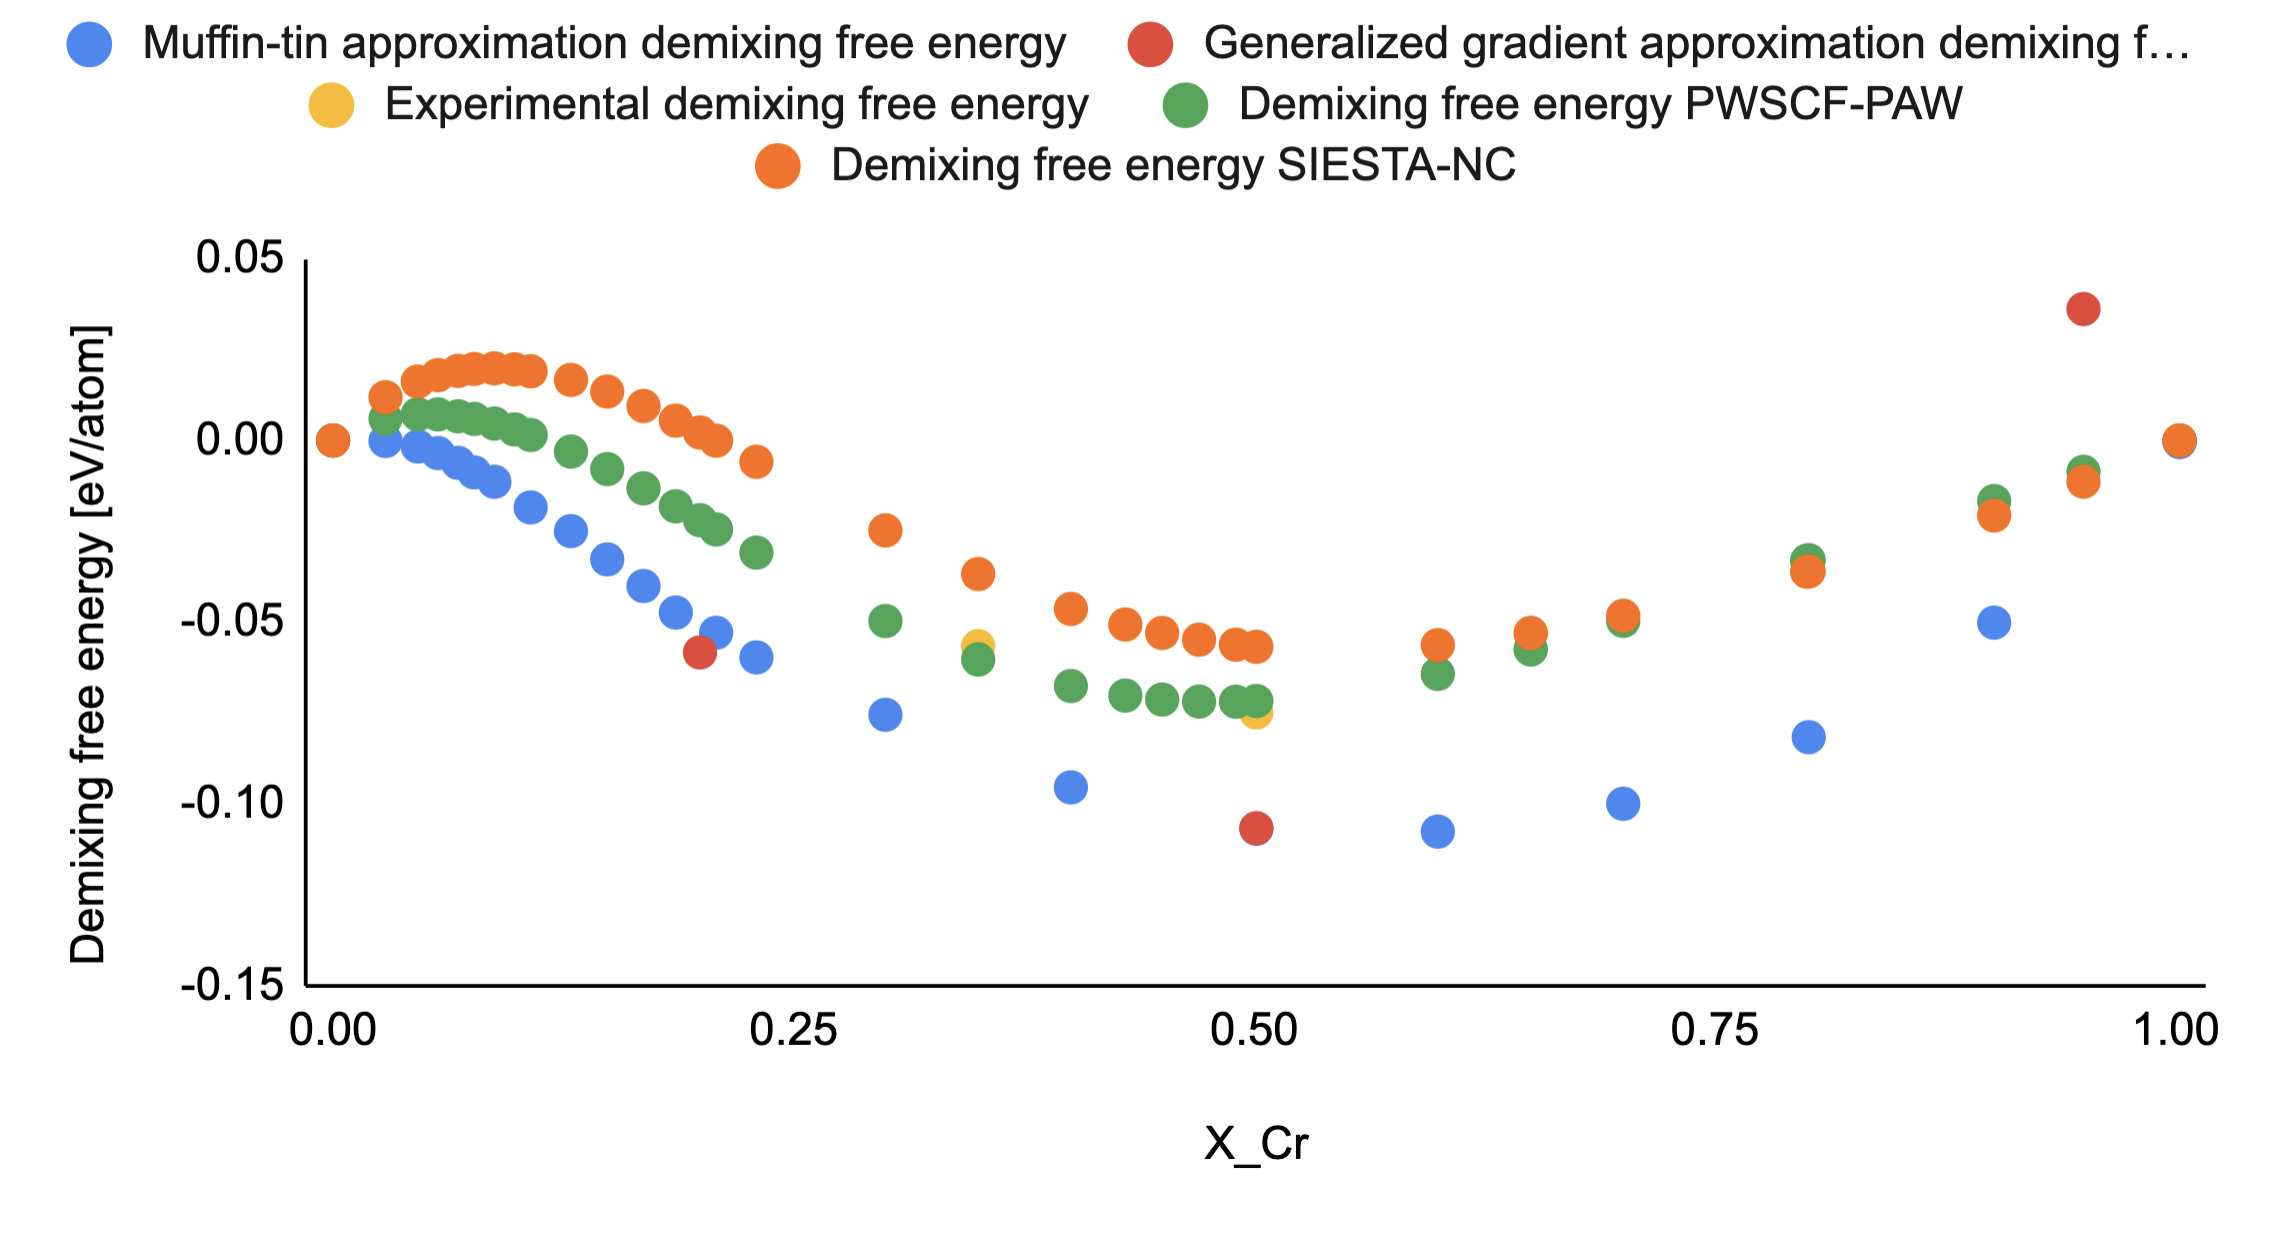
\includegraphics[width=\linewidth]{figures/dG_fig0a.png}
\end{subfigure}\hfill
\begin{subfigure}{0.48\linewidth}
    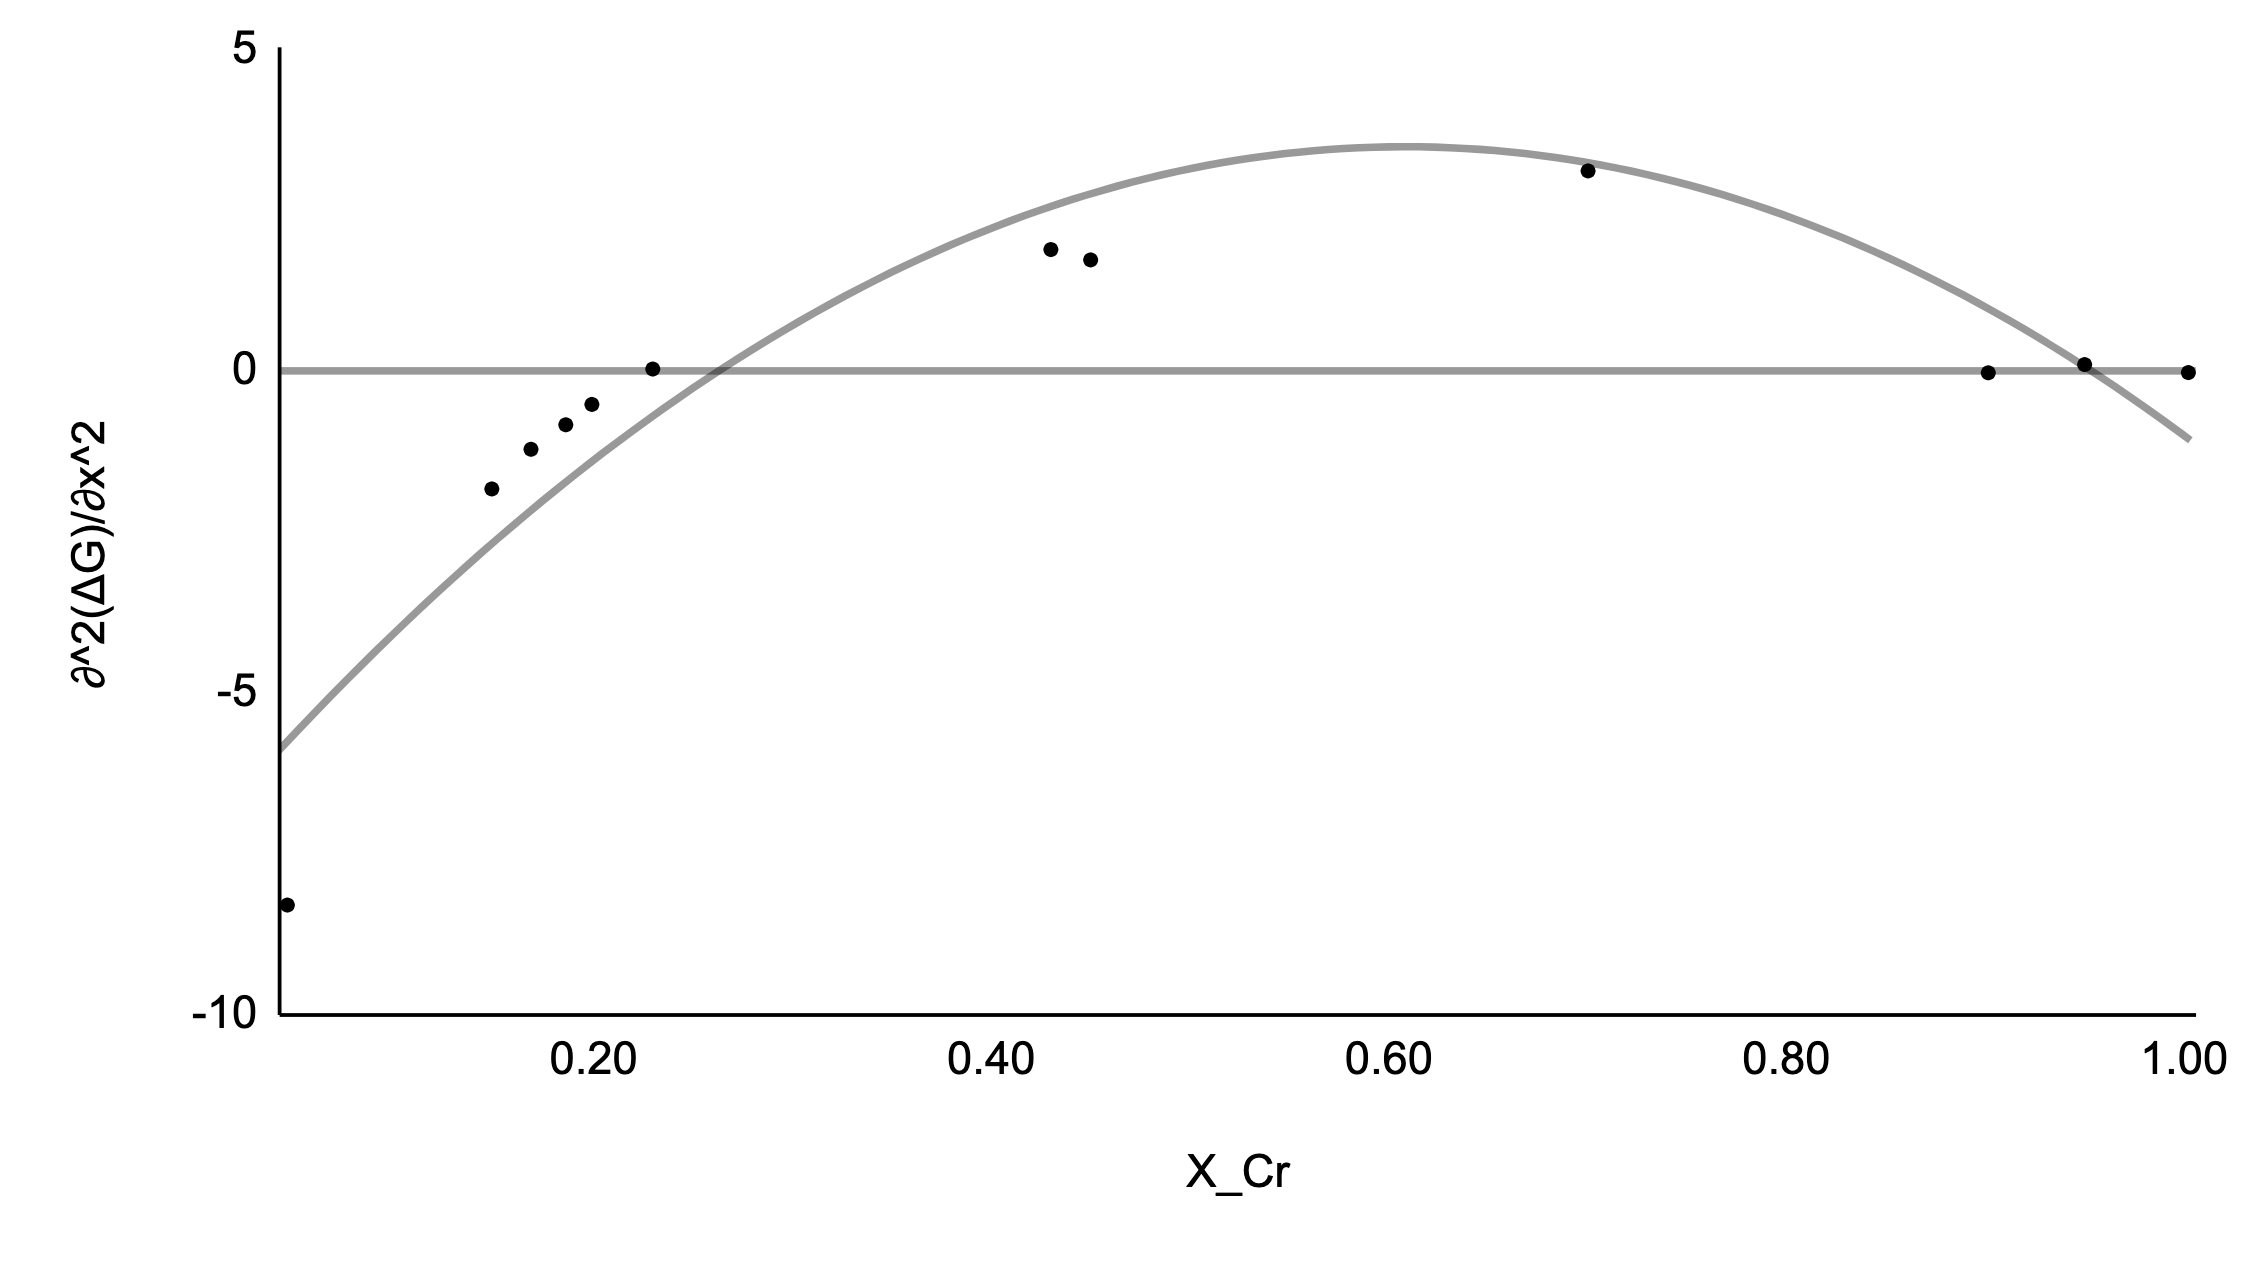
\includegraphics[width=\linewidth]{figures/ddGddx_fig0b.png}
\end{subfigure}
\caption{(a) Demixing free energy $\Delta G$ versus chromium composition $x_{\mathrm{Cr}}$. 
(b) Curvature $\partial^2 \Delta G/\partial x_{\mathrm{Cr}}^2$, identifying spinodally unstable composition windows where the curvature becomes negative.}
\label{fig:free_energy}
\end{figure}

Figure~\ref{fig:free_energy} shows that the onset of negative curvature occurs over a finite range of chromium compositions relevant to $\delta$--ferrite in stainless steels. This thermodynamic instability defines the regime in which elastic and acoustic properties cannot be interpreted assuming a homogeneous solid solution. Instead, any observable elastic response must be understood as emerging from a system that is intrinsically driven toward compositional modulation, providing the foundation for linking free-energy curvature to stiffness evolution and ultimately to ultrasonic observables.

\subsection{Elastic stiffening and elastodynamic mapping to Rayleigh SAW observables}

% --- FIGURE: elasticity + elastodynamics ---
\begin{figure}[!h]
\centering
\begin{subfigure}{0.48\linewidth}
    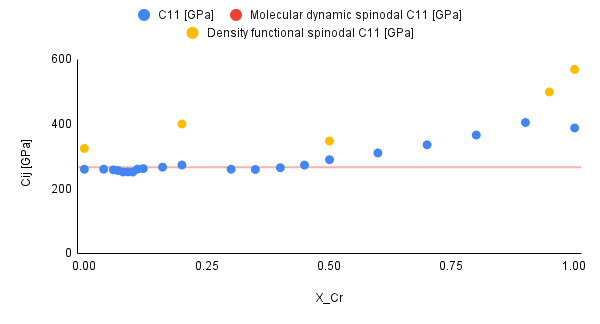
\includegraphics[width=\linewidth]{figures/Fe(1-x)Crx bcc cubic elastic tensor_fig1.png}
\end{subfigure}\hfill
\begin{subfigure}{0.48\linewidth}
    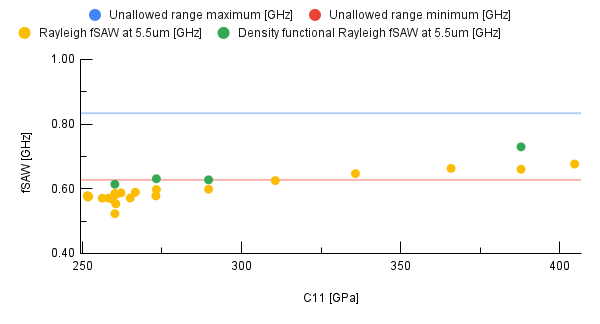
\includegraphics[width=\linewidth]{figures/Fe(1-x)Crx bcc cubic elastodynamics_fig2_ours.png}
\end{subfigure}
\caption{(a) Composition dependence of the bcc Fe$_{1-x}$Cr$_x$ cubic elastic tensor, shown for the longitudinal stiffness $C_{11}$. 
(b) Elastodynamic mapping from elastic stiffness to Rayleigh surface acoustic wave frequency $f_{\mathrm{SAW}}$, indicating elastodynamically allowed and unallowed frequency ranges for a homogeneous solid solution.}
\label{fig:elastic_elastodynamics}
\end{figure}

To connect thermodynamic instability to experimentally measurable quantities, we compute the cubic elastic tensor across $x_{\mathrm{Cr}}$ and propagate these elastic inputs through elastodynamic constraints relevant to surface acoustic waves. In the present geometry, the longitudinal stiffness component $C_{11}$ plays a dominant role in controlling the Rayleigh SAW frequency through the dispersion relation, making it a sensitive indicator of composition-dependent stiffening. Small overpredictions in absolute frequency are attributed to finite-size SQS representations and the absence of magnetic and chemical short-range order beyond the supercell length scale. Importantly, relative stiffening trends and peak splitting remain robust, demonstrating that first-principles elasticity captures the essential physics governing SAW observables.




As shown in Fig.~\ref{fig:elastic_elastodynamics}, $C_{11}$ exhibits a systematic dependence on chromium concentration, producing corresponding shifts in the elastodynamically allowed Rayleigh SAW frequency range. Importantly, this mapping provides a quantitative bridge between first-principles elasticity and experimentally observed SAW peak positions. Within the spinodally unstable composition window, elastic stiffening therefore translates directly into measurable acoustic signatures, enabling stiffness changes to be inferred non-destructively.

\subsection{Separating composition trends from spinodal conversion trends}

While elastic constants vary with chromium concentration even in a homogeneous solid solution, spinodal decomposition introduces an additional, time-dependent microstructural evolution. To disentangle these effects, it is necessary to distinguish changes driven purely by composition from those arising from the progression of phase separation. We therefore report two complementary relationships that isolate these contributions within a unified elastodynamic framework.

% --- FIGURE: fSAW vs xCr and vs phi ---
\begin{figure}[!h]
\centering
\begin{subfigure}{0.48\linewidth}
    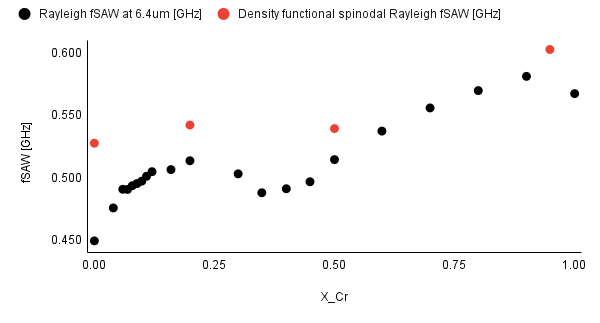
\includegraphics[width=\linewidth]{figures/Rayleigh fSAW [GHz] vs. X_Cr only_fig3.png}
\end{subfigure}\hfill
\begin{subfigure}{0.48\linewidth}
    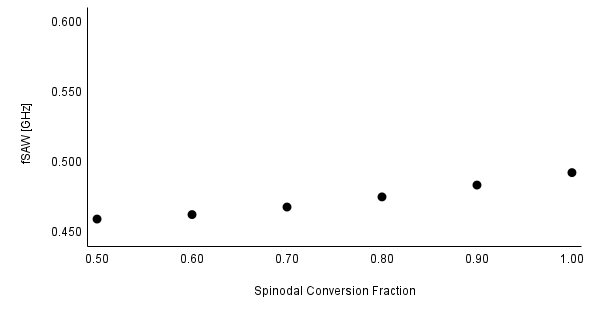
\includegraphics[width=\linewidth]{figures/Rayleigh fSAW [GHz] vs. Spinodal Conversion Fraction only_fig4.png}
\end{subfigure}
\caption{(a) Rayleigh SAW frequency $f_{\mathrm{SAW}}$ as a function of chromium composition $x_{\mathrm{Cr}}$ using DFT-derived elastic constants (solid-solution trend). 
(b) Rayleigh SAW frequency as a function of spinodal conversion fraction $\phi$ from molecular dynamics, isolating microstructural evolution effects during decomposition.}
\label{fig:fsaw_combined}
\end{figure}

Figure~\ref{fig:fsaw_combined} demonstrates that while $f_{\mathrm{SAW}}(x_{\mathrm{Cr}})$ captures the baseline elastic response of a homogeneous alloy, the evolution of $f_{\mathrm{SAW}}(\phi)$ reflects additional stiffening associated with progressive spinodal conversion. This separation enables experimental SAW measurements to be interpreted in terms of both composition and decomposition state, providing a pathway to distinguish early-stage spinodal evolution from equilibrium compositional effects.


\section{Discussion}

Taken together, the results establish a closed thermodynamics-to-observable pathway for interpreting picosecond ultrasonic measurements in $\delta$--ferrite–containing stainless steels. The free-energy curvature criterion identifies the composition window in which the homogeneous solid solution is intrinsically unstable, defining the regime where elastic and acoustic properties must reflect ongoing or incipient spinodal decomposition rather than equilibrium alloy behavior.

Within this thermodynamically unstable regime, first-principles elasticity reveals systematic stiffening trends that are propagated through elastodynamic constraints into Rayleigh SAW frequency shifts. The direct mapping between elastic constants and SAW observables provides a quantitative basis for interpreting peak shifts and splitting as signatures of stiffness evolution, rather than purely phenomenological indicators.

Crucially, separating the solid-solution trend $f_{\mathrm{SAW}}(x_{\mathrm{Cr}})$ from the spinodal conversion trend $f_{\mathrm{SAW}}(\phi)$ resolves a key ambiguity in experimental interpretation. While composition alone can shift SAW frequencies, progressive spinodal decomposition introduces additional stiffening that cannot be captured by composition-dependent elasticity alone. The combined framework therefore enables SAW peak splitting to be interpreted as a mechanistically grounded indicator of microstructural evolution toward embrittlement, rather than as a purely compositional effect.

This separation clarifies why SAW peak splitting emerges as a robust, non-destructive diagnostic of spinodal decomposition in CASS and related alloys, and suggests a general strategy for extending ultrasonic embrittlement detection to other phase-separating structural materials.




\section{Conclusions}
We presented a compact thermodynamics-to-elastodynamics workflow for bcc Fe--Cr $\delta$--ferrite that links demixing free-energy curvature, first-principles elastic constants, and Rayleigh SAW observables. Free-energy curvature provides a direct stability criterion that identifies spinodally unstable composition windows. DFT-derived cubic elasticity quantifies composition-dependent stiffening trends and supplies inputs for elastodynamic prediction. Combining these elements yields experimentally actionable relationships for interpreting picosecond ultrasonics across both composition and decomposition-state variables.


\bibliographystyle{elsarticle-num}
\bibliography{references}


\newpage
\clearpage

\section*{Supplementary Material}
The following material retains the original draft figures for completeness and traceability. All figure numbering in this supplementary section is independent of the main manuscript.

\setcounter{figure}{0}
\renewcommand{\thefigure}{S\arabic{figure}}


\begin{figure}[!ht]
\centering
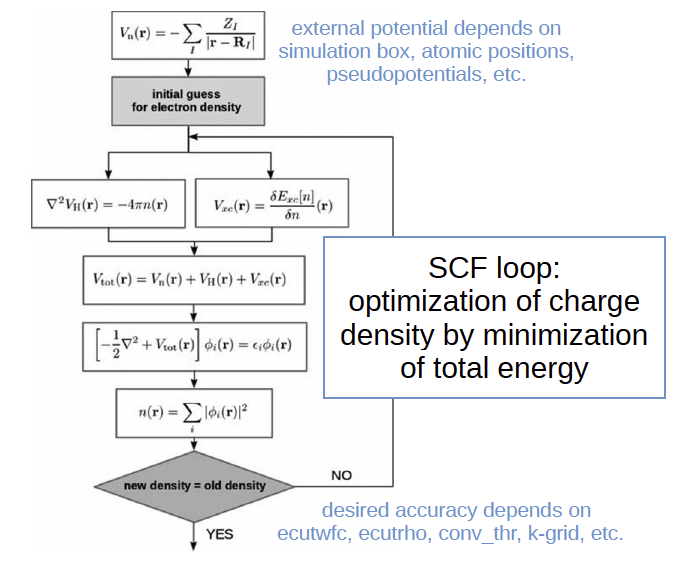
\includegraphics[width=0.85\textwidth]{figures/SCF.png}
\caption{SCF loop schematic illustrating self-consistent electronic-structure workflow \cite{giustino2014materials}.}
\label{fig:SCF-loop}
\end{figure}


\begin{figure}[h!]
    \centering
    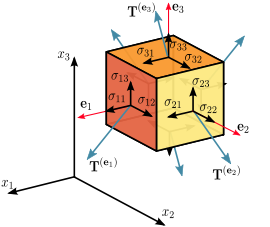
\includegraphics[width=0.6\textwidth]{Parts/Figures/Cij.png}
    \caption{Stress tensor visualization \cite{al2020non}.}
    \label{fig:seis-refl-tech}
\end{figure}

\begin{figure}[!ht]
	\centering
	\begin{subfigure}{0.9\textwidth}
         \centering
         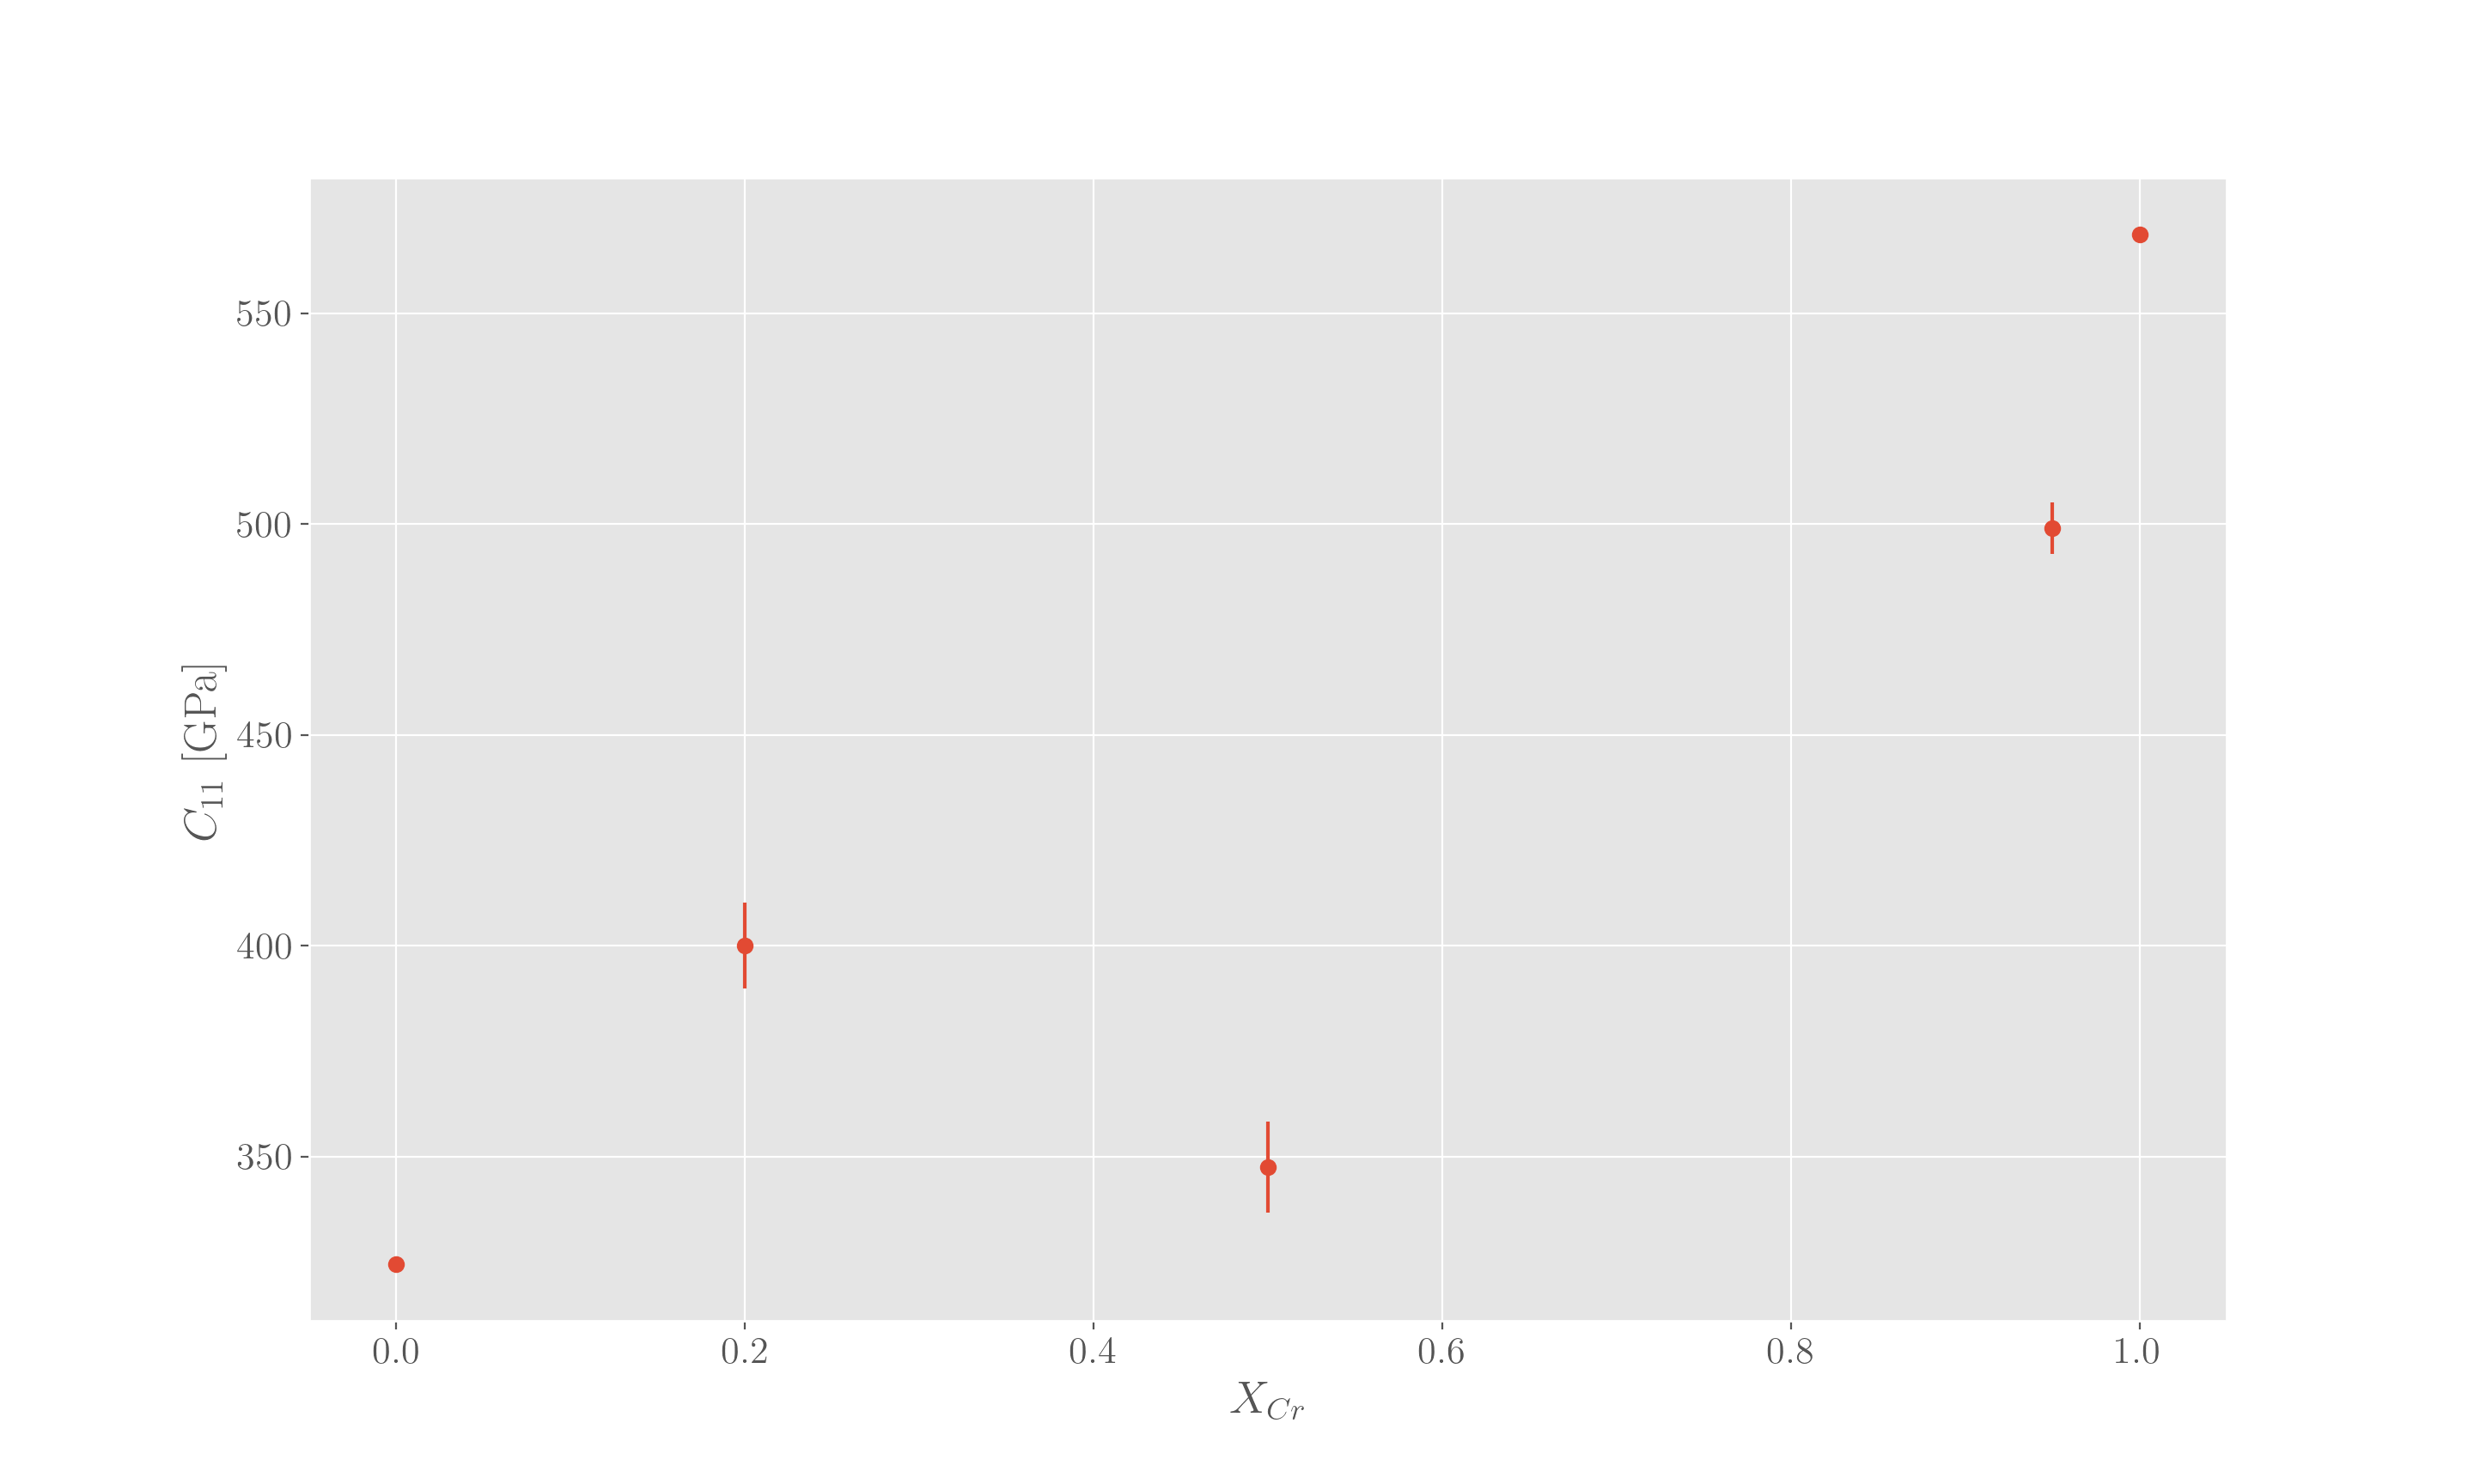
\includegraphics[width=\linewidth]{Parts/Figures/C11.png}
         \caption{Normal constant, \(C_{11}\), illustrating the longitudinal stiffness of bcc binary FeCr alloy as a function of chromium composition. This stiffness parameter is crucial for understanding the acoustic velocity and mechanical properties of the material.}
         \label{fig1a}
     \end{subfigure}
     \hfill
     \begin{subfigure}{0.45\textwidth}
         \centering
         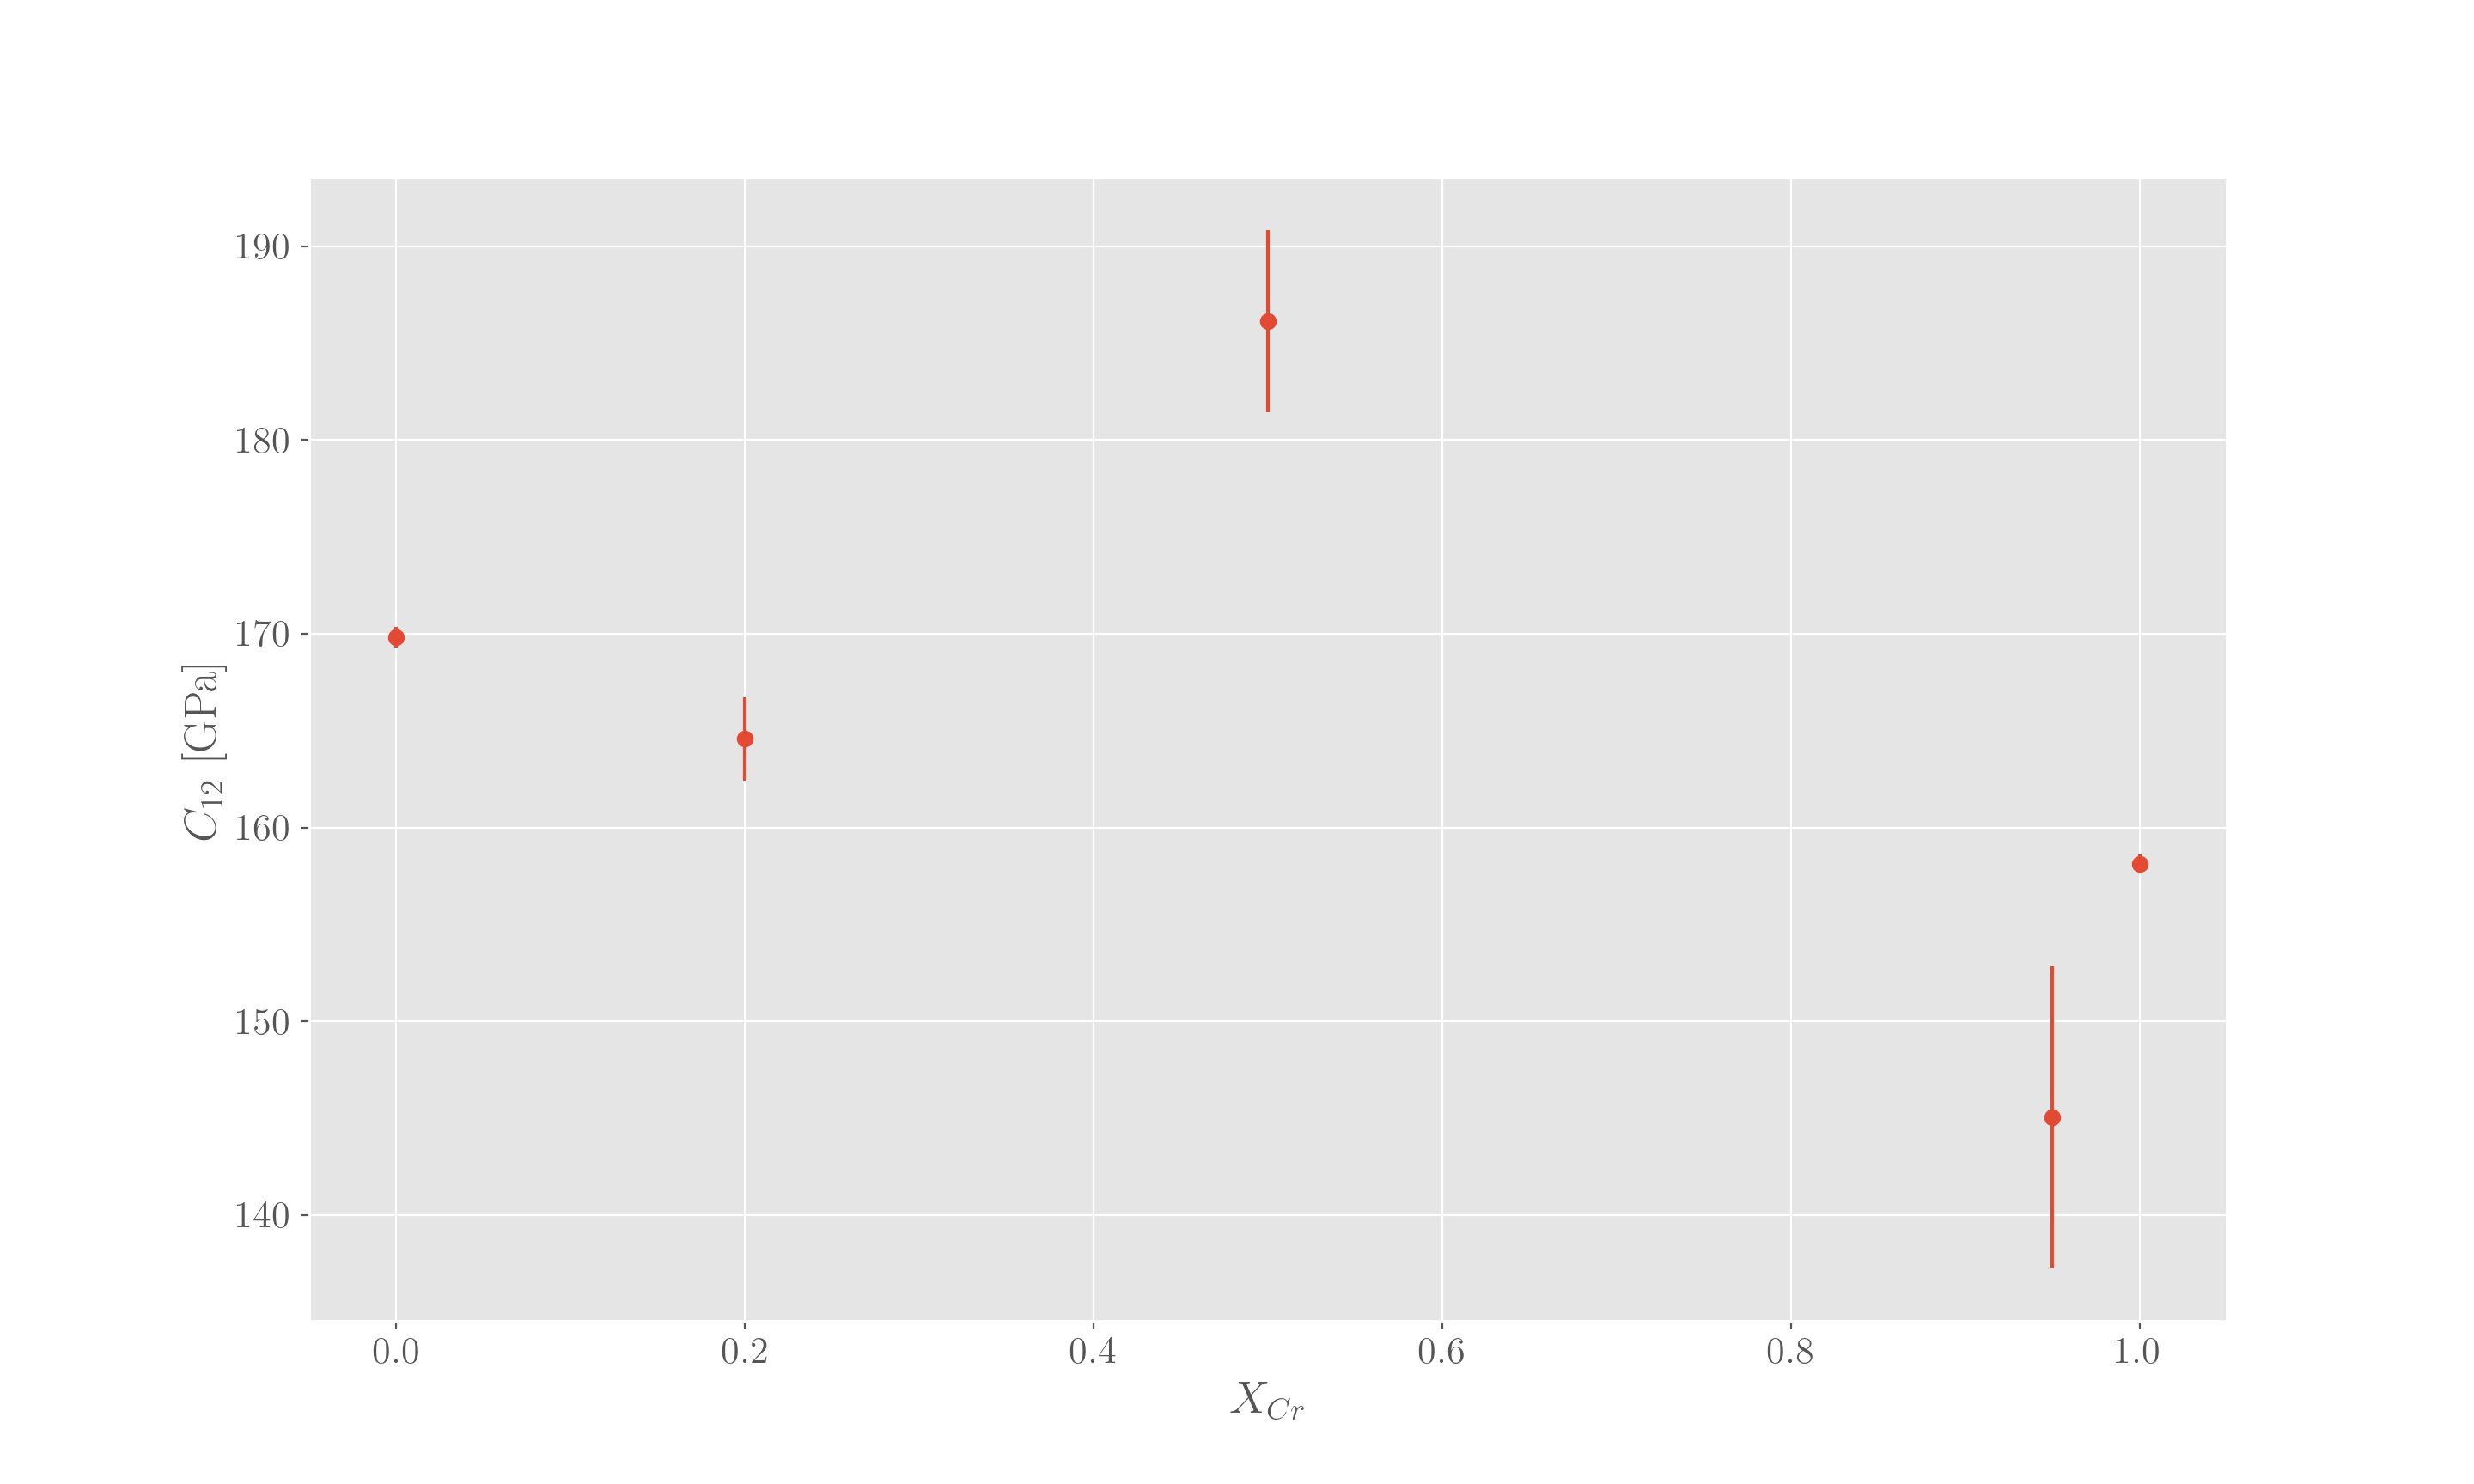
\includegraphics[width=\linewidth]{Parts/Figures/C12.png}
         \caption{The interplanar elastic constant \(C_{12}\), showing the coupling between axial and lateral strains, indicative of the alloy's resistance to shear along crystallographic planes.}
         \label{fig1b}
     \end{subfigure}
     \hfill
     \begin{subfigure}{0.45\textwidth}
         \centering
         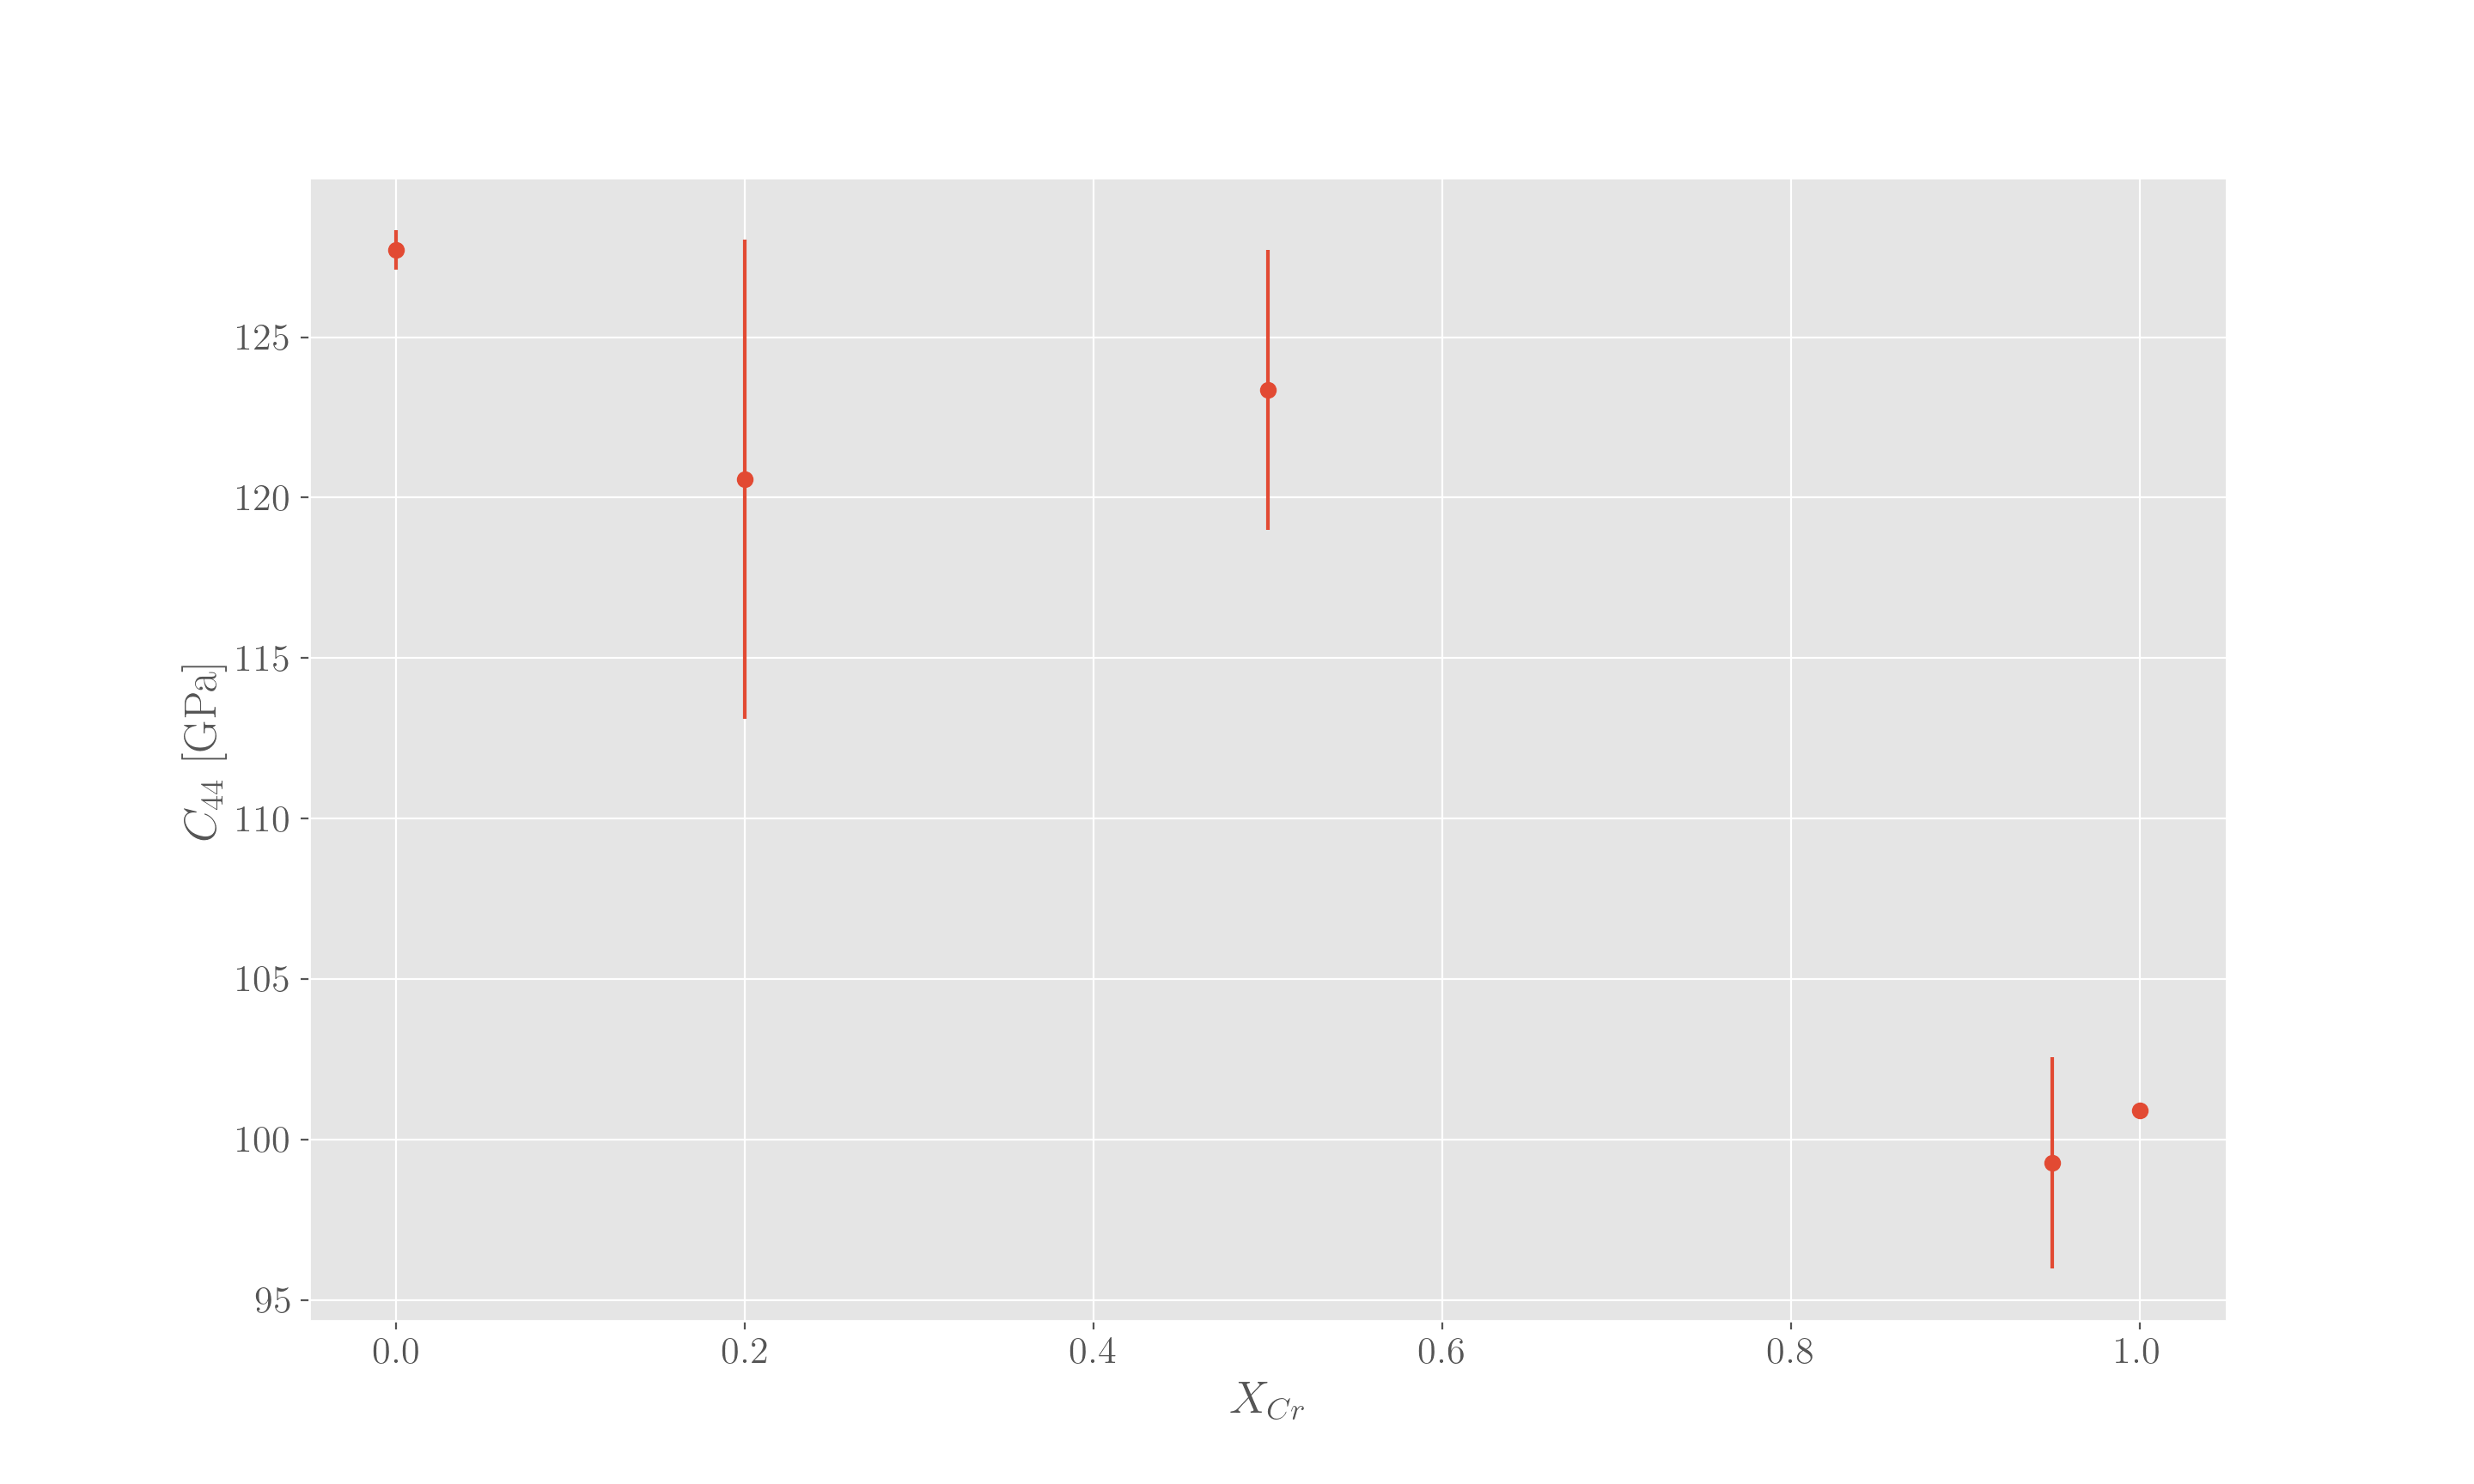
\includegraphics[width=\linewidth]{Parts/Figures/C44.png}
         \caption{Shear constant, \(C_{44}\), representing shear stiffness against deformation without volume change, critical for assessing material's resistance to applied shear stress.}
         \label{fig1c}
     \end{subfigure}
	\caption{Elastic constants of bcc binary FeCr as a function of Cr composition indicate spinodal decomposition-induced stiffening towards embrittlement. The trends and values are consistent with theoretical and experimental results reported in literature. (a) Shows the longitudinal stiffness parameter \(C_{11}\), important for evaluating the material's response to compressive and tensile stresses. (b) Highlights \(C_{12}\), which is essential for understanding the coupling between different types of strain. (c) Details \(C_{44}\), crucial for evaluating the shear deformation behavior.}
	\label{fig1}
\end{figure}


\begin{figure}[!ht]
	\centering
	\begin{subfigure}{0.9\textwidth}
         \centering
         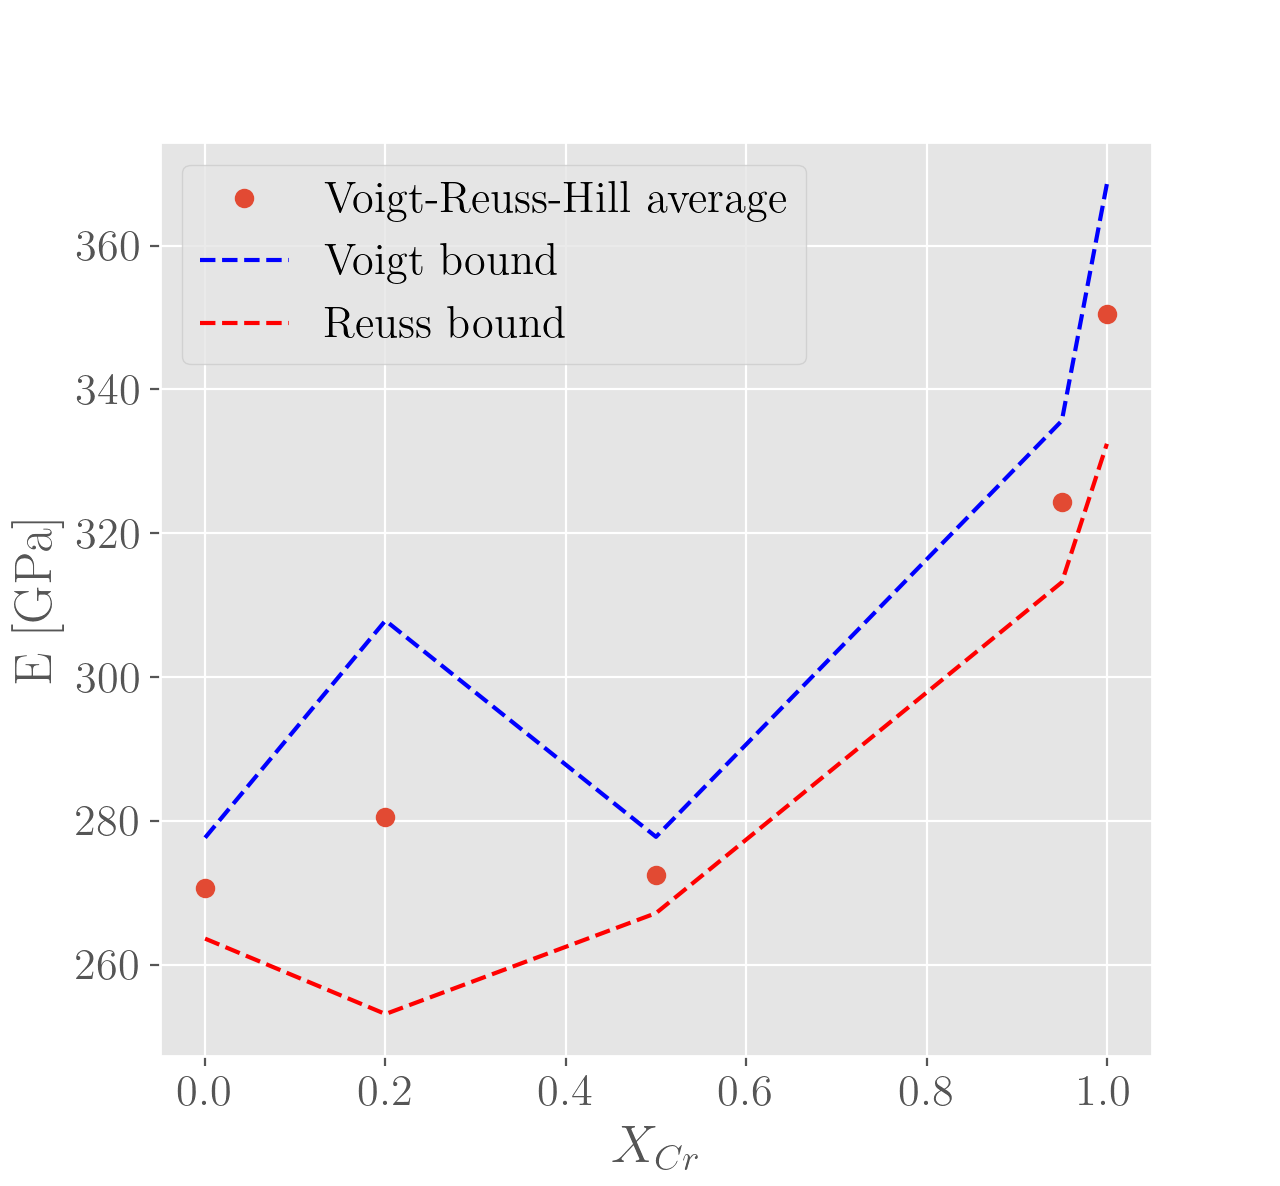
\includegraphics[width=0.9\linewidth]{Parts/Figures/E_VRH.png}
         \caption{Elastic (Young's) Modulus, \(E_{VRH}\), indicating the material's stiffness and its ability to resist deformation under tensile stress.}
         \label{fig2a}
     \end{subfigure}
     \hfill
     \begin{subfigure}{0.45\textwidth}
         \centering
         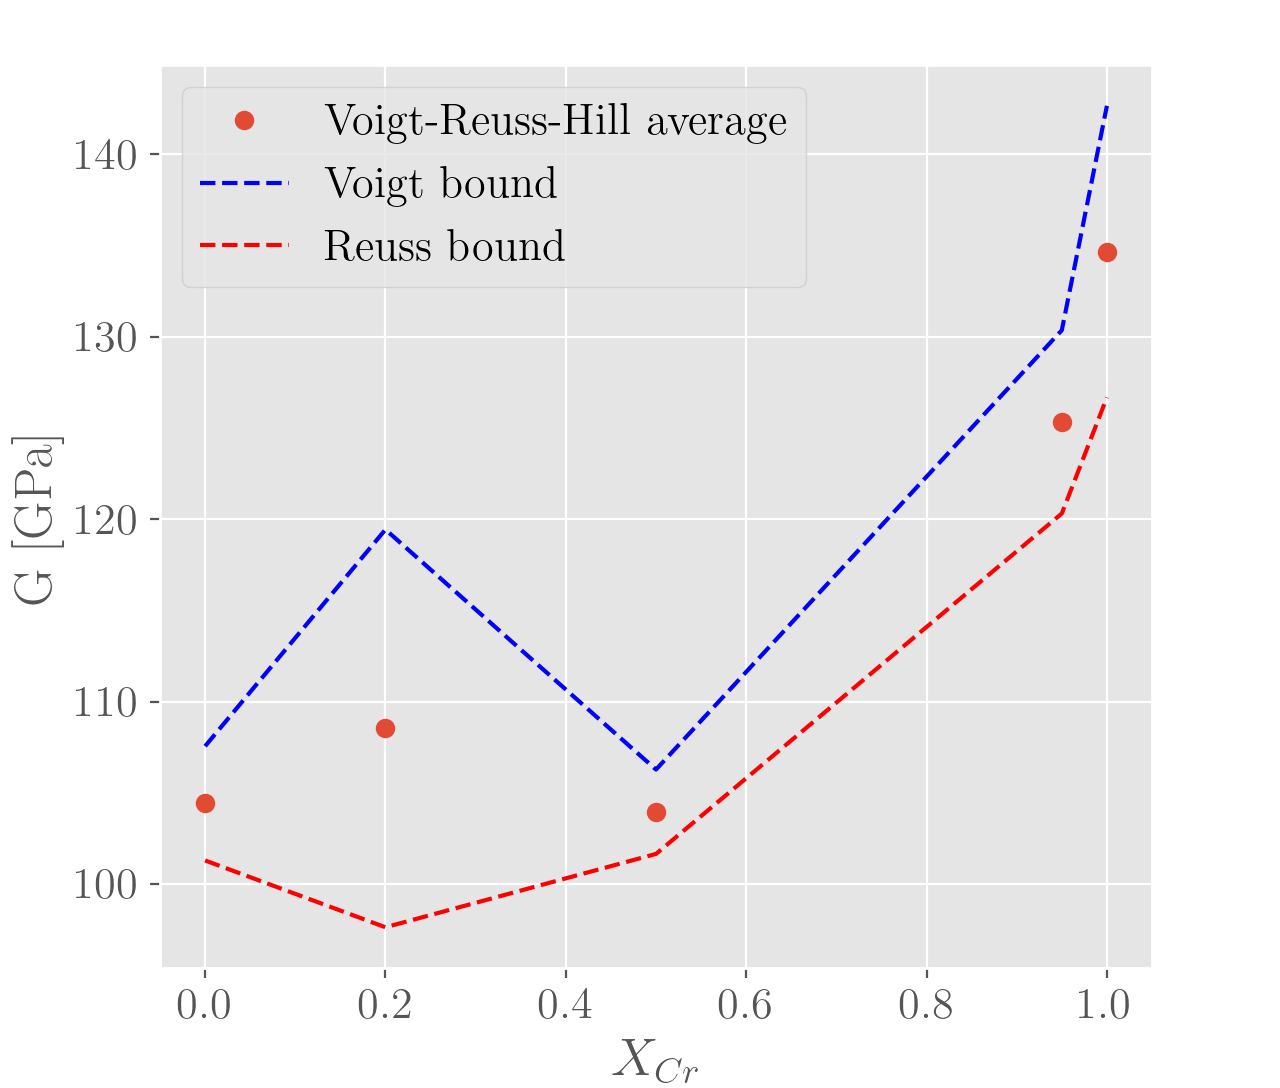
\includegraphics[width=\linewidth]{Parts/Figures/G_VRH.png}
         \caption{Shear modulus, \(G_{VRH}\), reflecting the material's ability to withstand shear deformation.}
         \label{fig2b}
     \end{subfigure}
     \hfill
     \begin{subfigure}{0.45\textwidth}
         \centering
         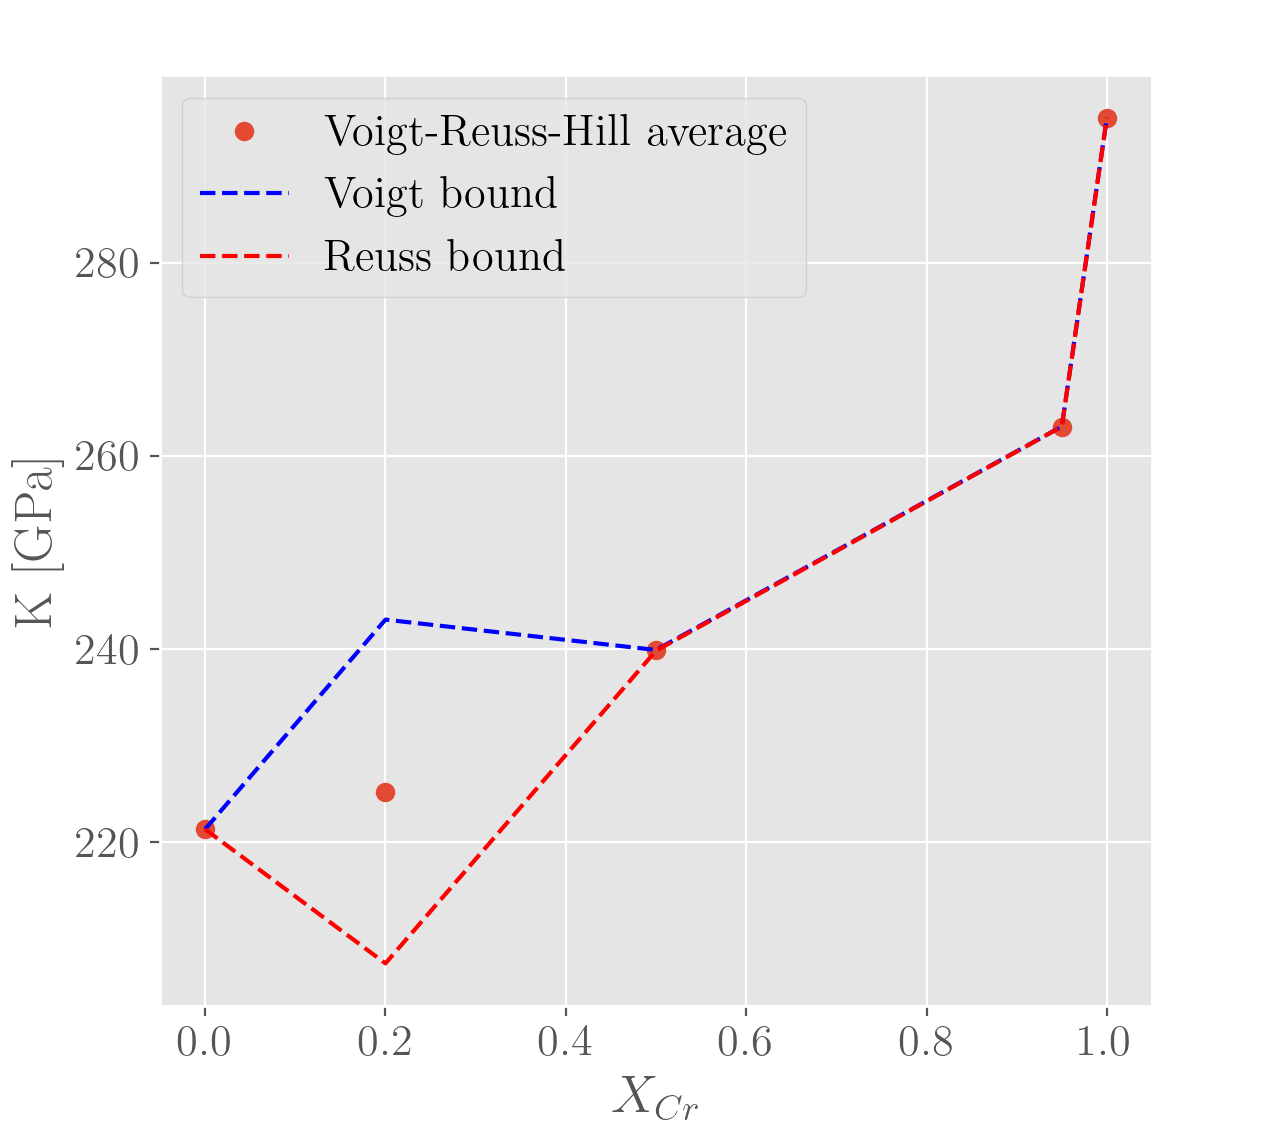
\includegraphics[width=\linewidth]{Parts/Figures/K_VRH.png}
         \caption{Bulk modulus, \(K_{VRH}\), which measures the material's resistance to uniform compression.}
         \label{fig2c}
     \end{subfigure}
	\caption{Elastic moduli of bcc binary FeCr as a function of Cr composition indicate spinodal decomposition-induced stiffening towards embrittlement. The trends and values are consistent with theoretical and experimental results reported in literature. (a) Elastic (Young's) Modulus demonstrates the material's overall stiffness. (b) Shear modulus is a measure of the alloy's rigidity against shear forces. (c) Bulk modulus assesses the material's compressibility under uniform pressure.}
	\label{fig2}
\end{figure}

\begin{sidewaysfigure}[!ht]
	\centering
	\begin{subfigure}{0.7\textwidth}
         \centering
         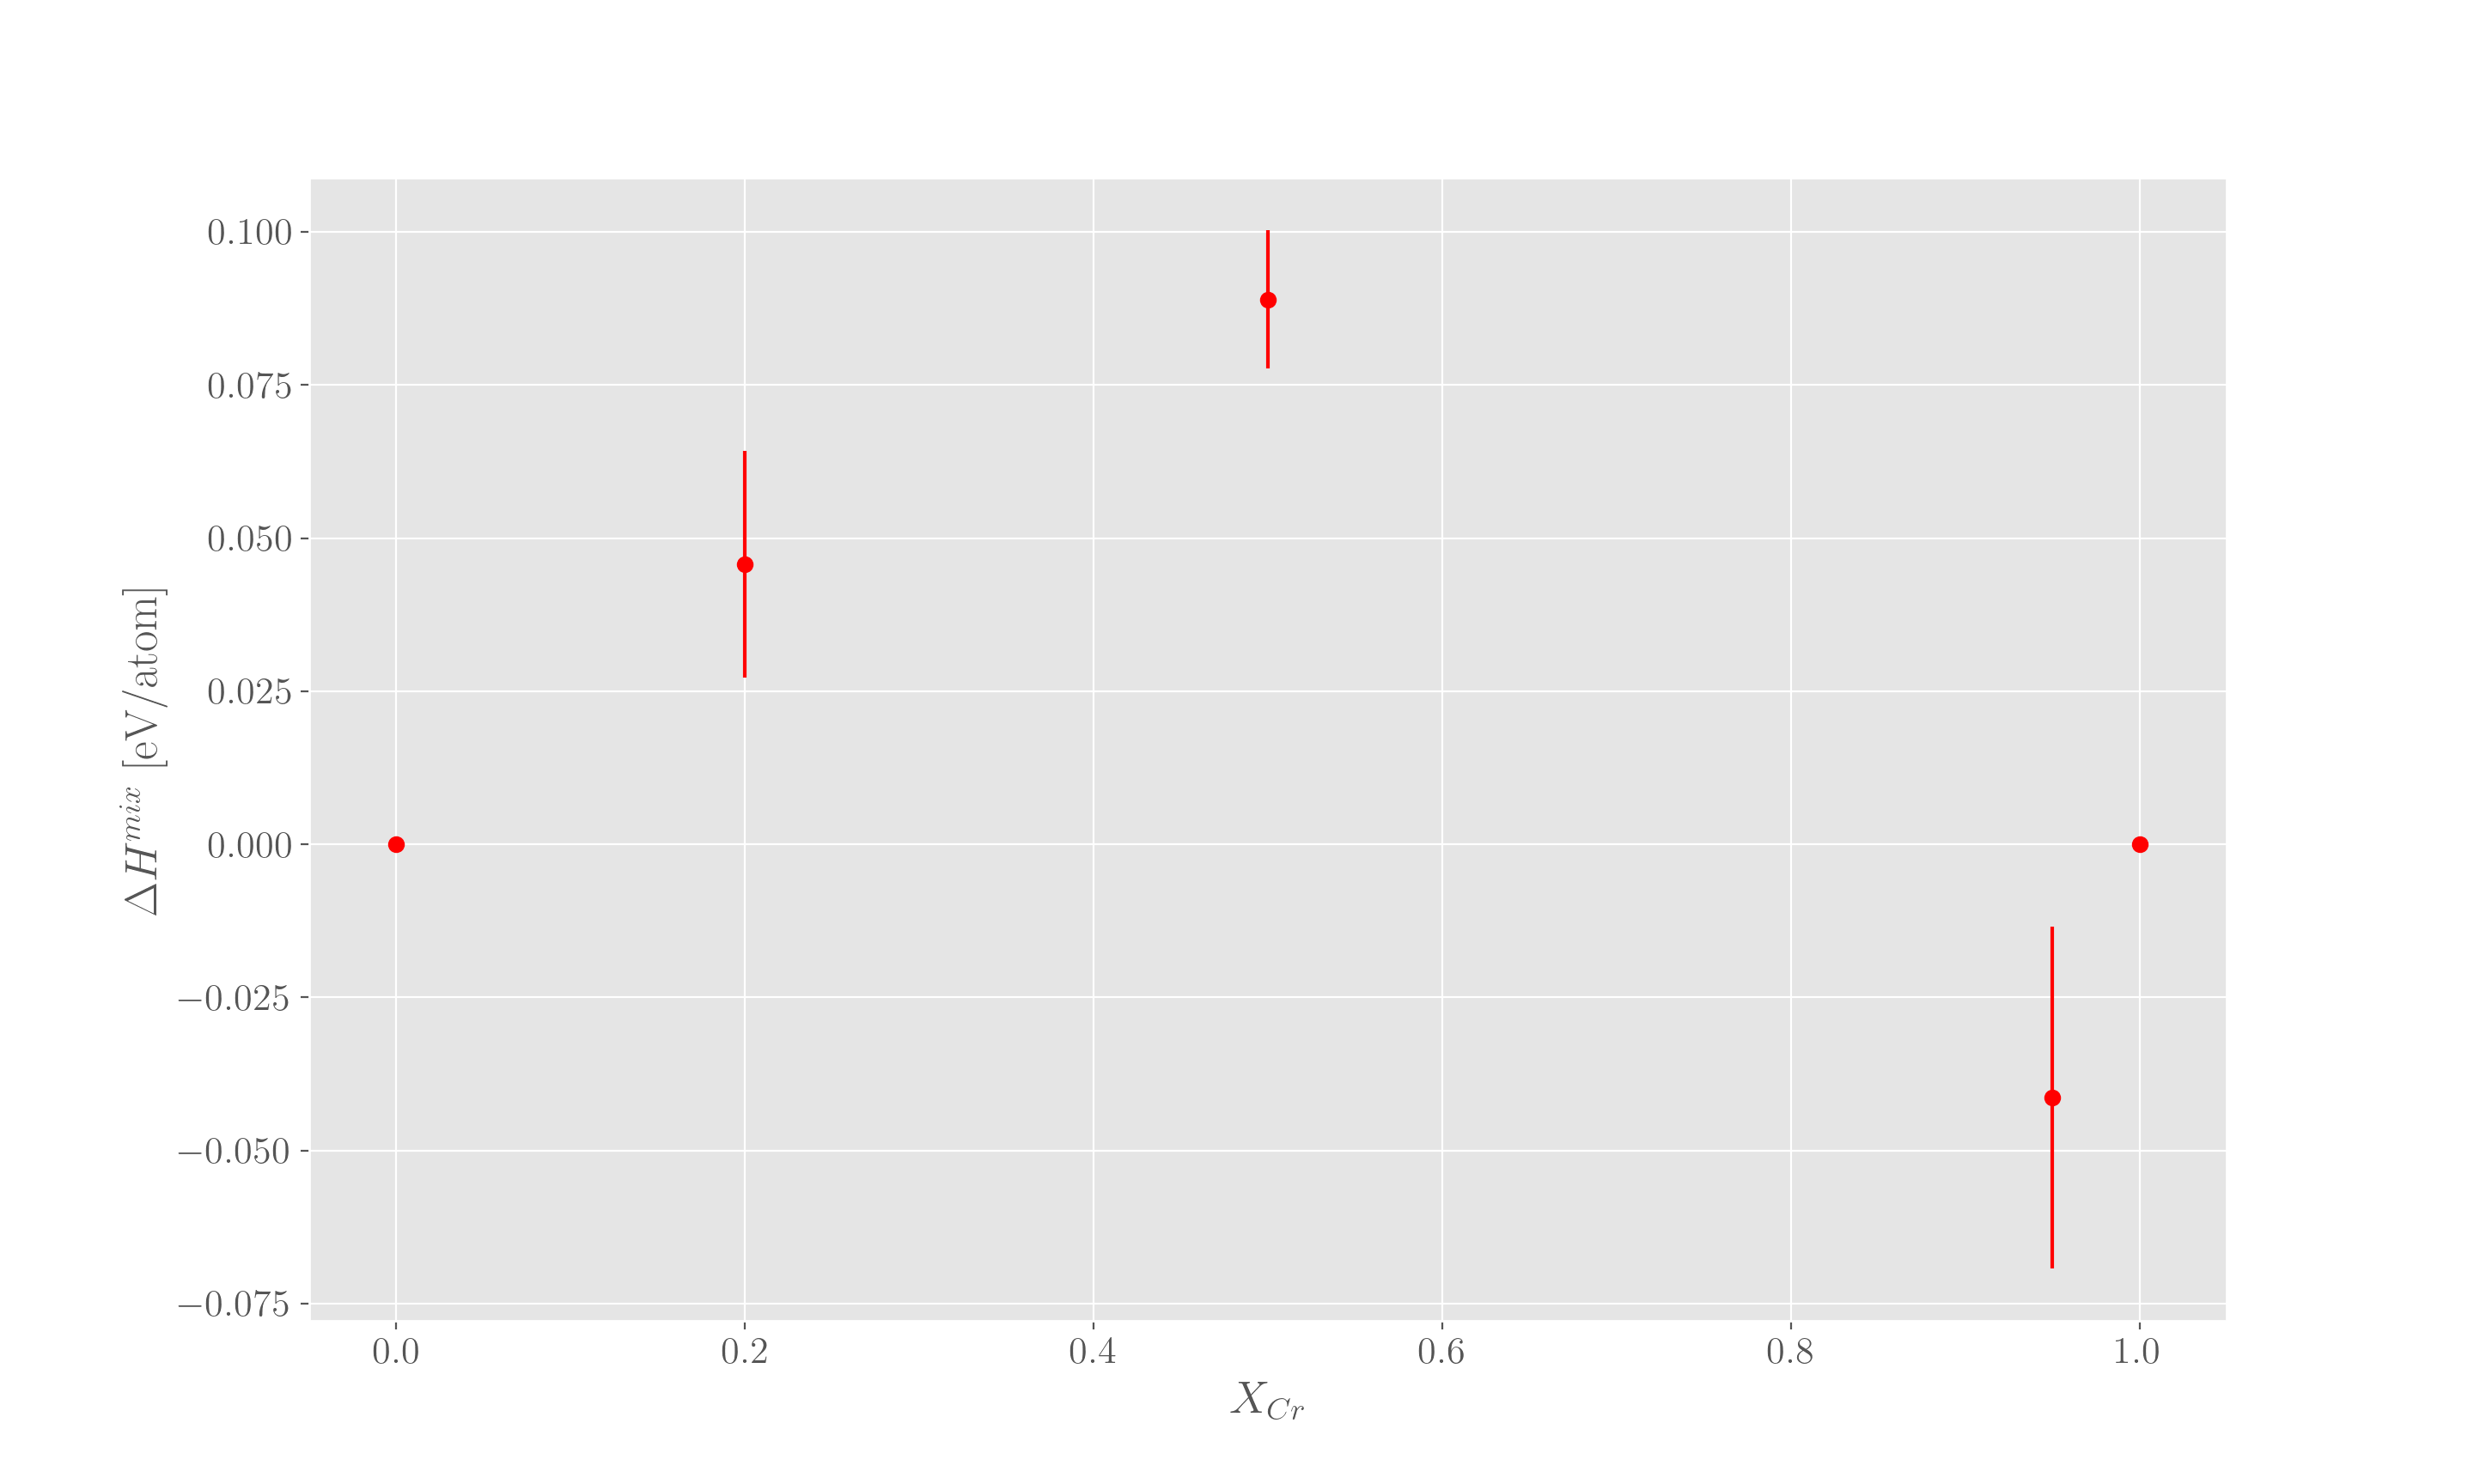
\includegraphics[width=\linewidth]{Parts/Figures/Hmix-vF.png}
         \caption{Enthalpy of mixing, showing the thermodynamic favorability of phase separation in bcc $\delta$-ferrite in cast austenitic stainless steels through spinodal decomposition.}
         \label{fig3a}
     \end{subfigure}
     \begin{subfigure}{0.3\textwidth}
         \centering
         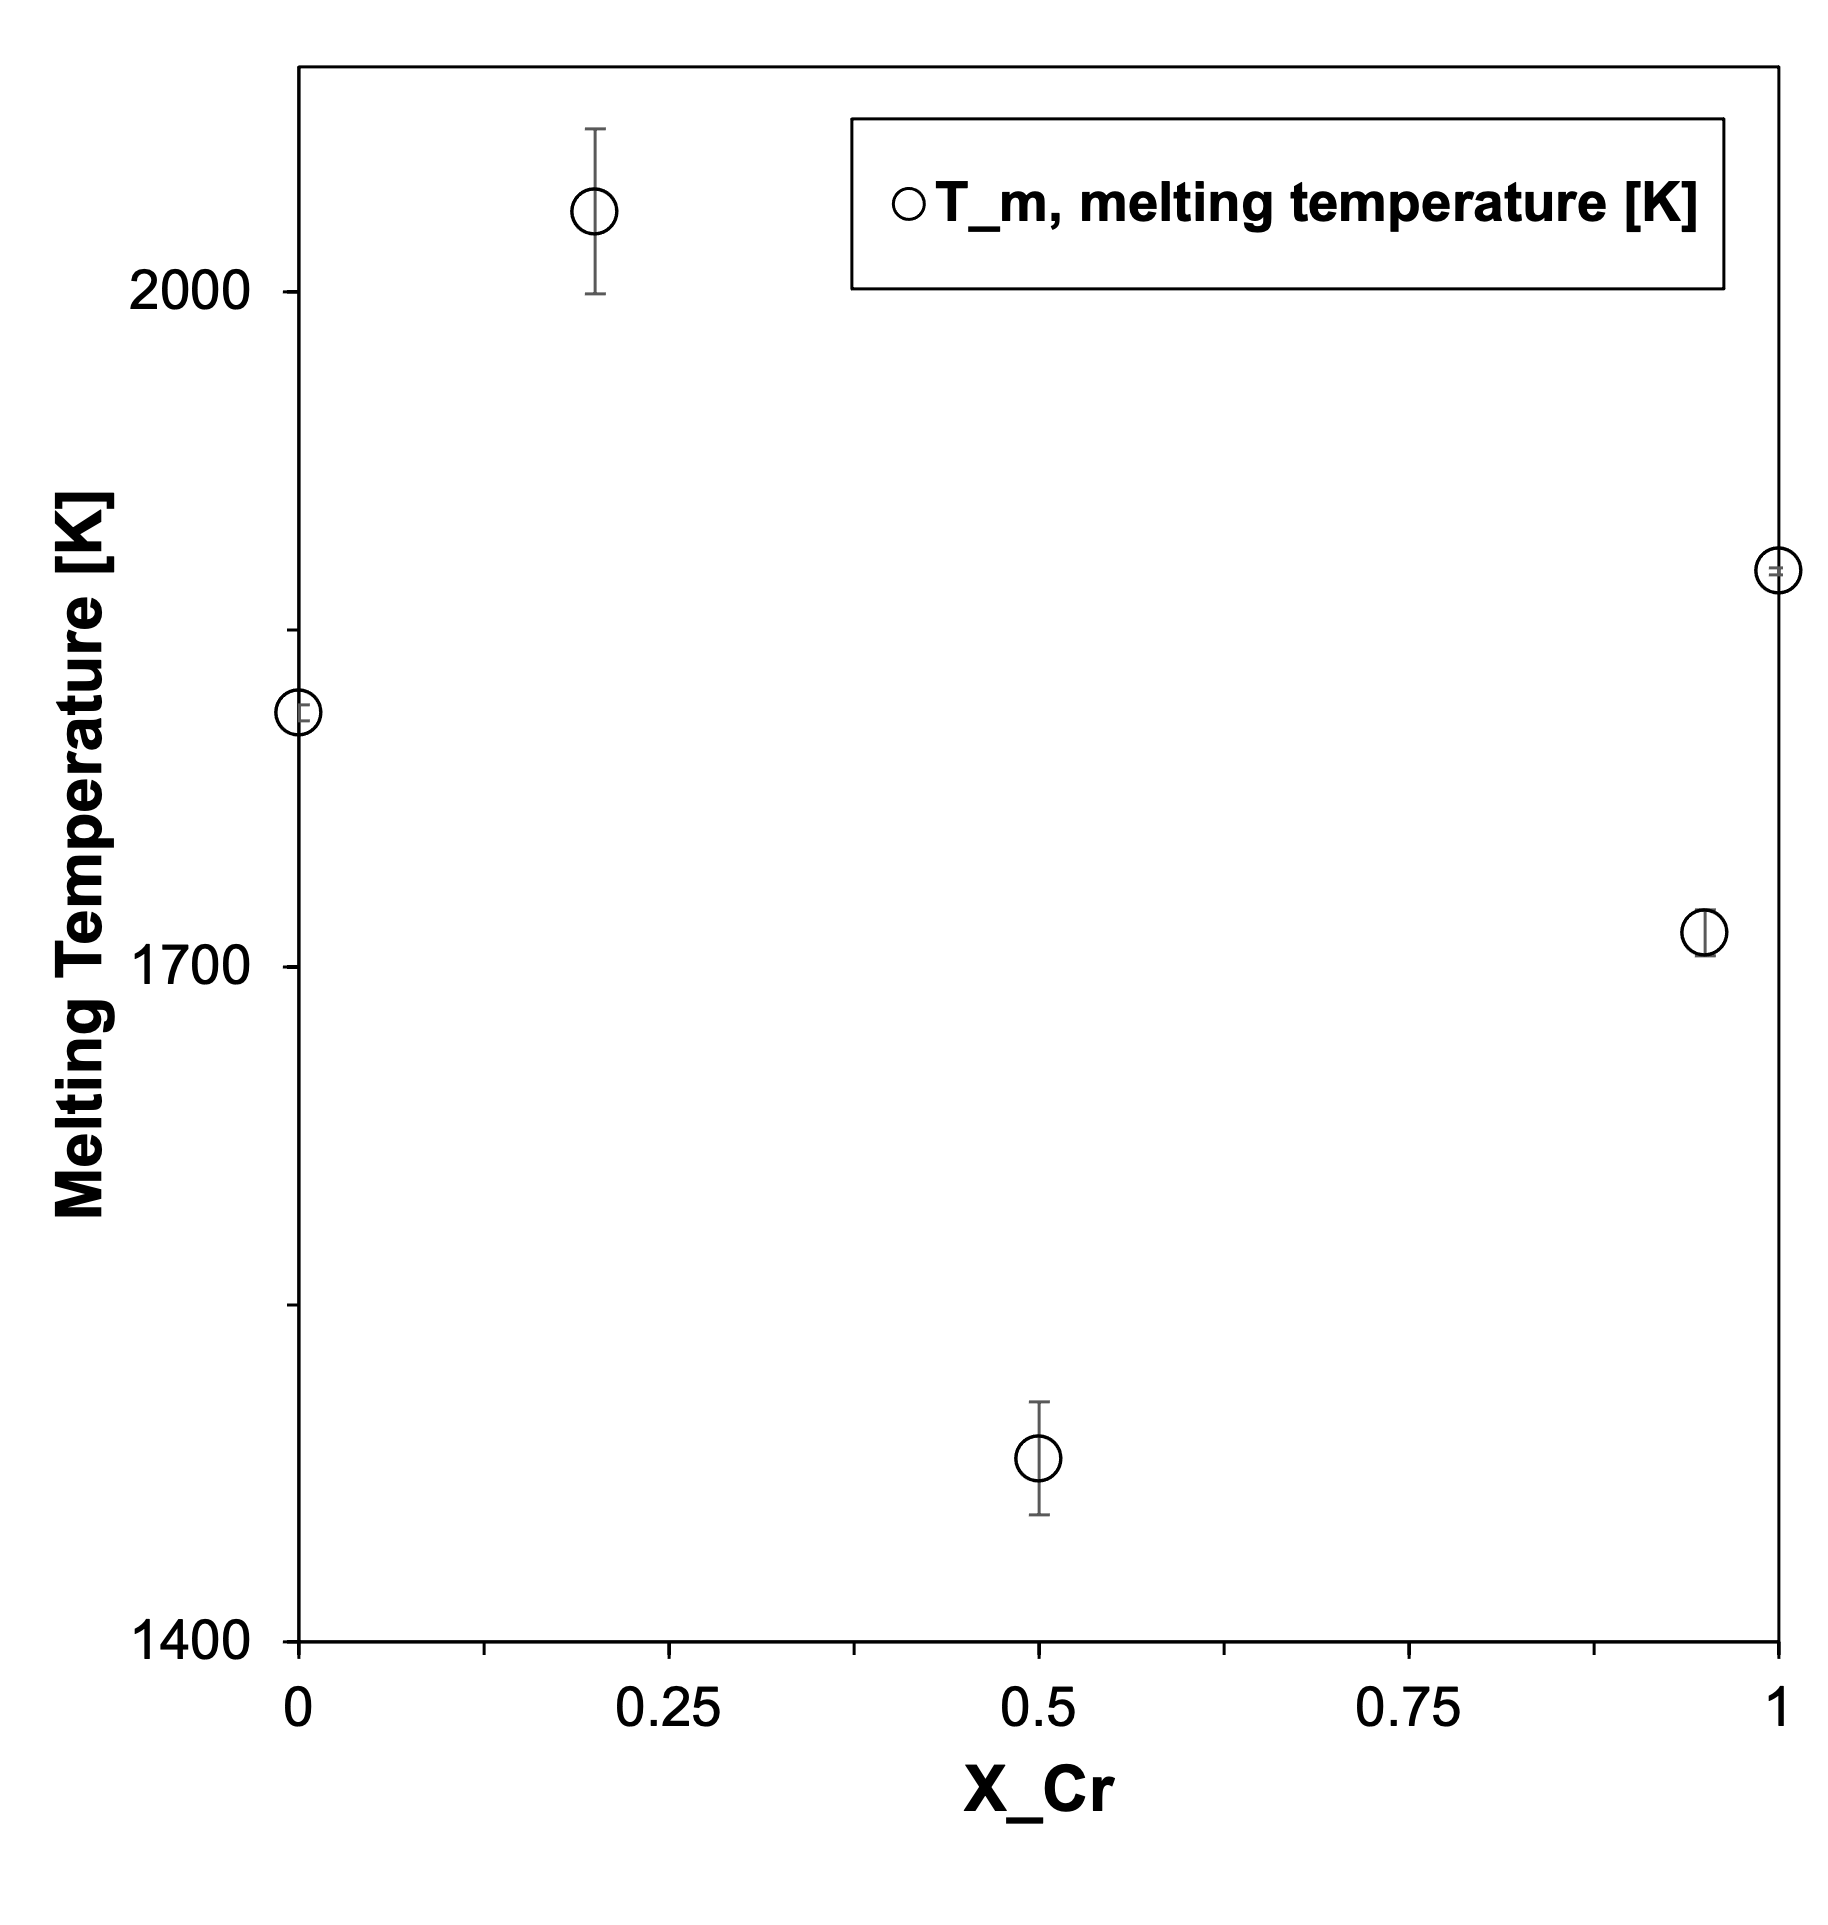
\includegraphics[width=\linewidth]{Parts/Figures/TMvsX_v2.png}
         \caption{\(T_M\), melting temperature, indicating how the thermal stability of the material changes with Cr composition.}
         \label{fig3b}
     \end{subfigure}
     \begin{subfigure}{0.3\textwidth}
         \centering
         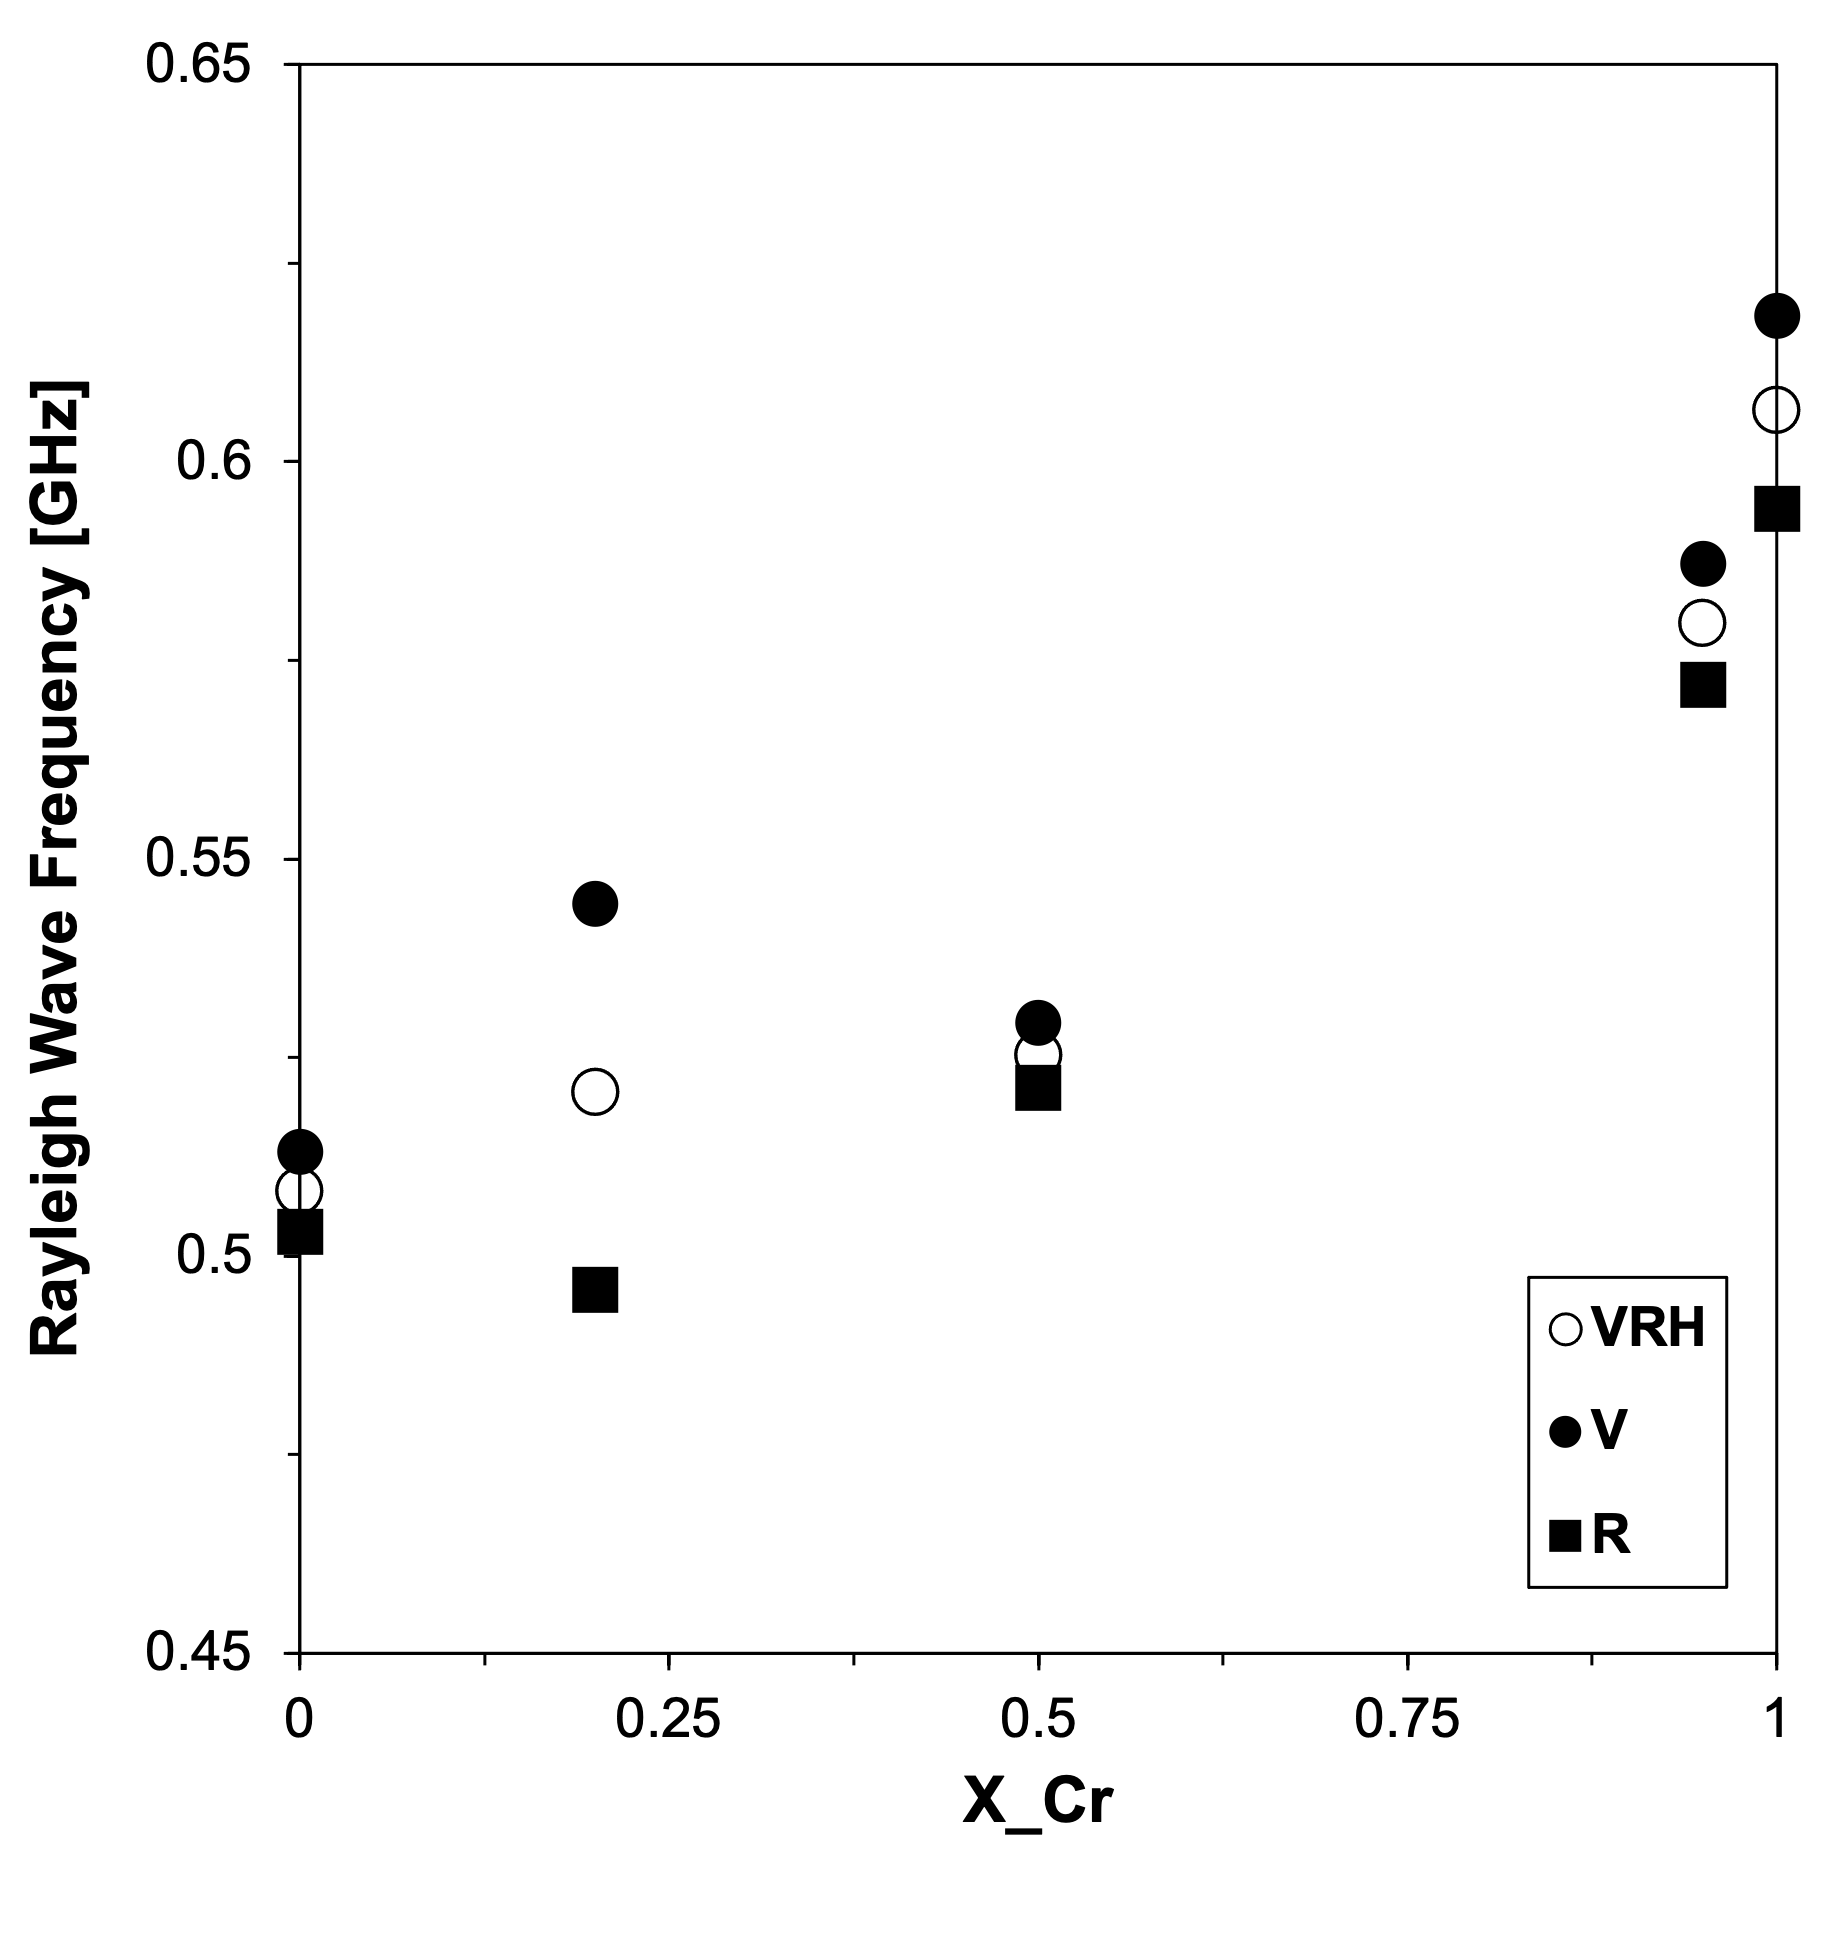
\includegraphics[width=\linewidth]{Parts/Figures/f_rwVsX_vF.png}
         \caption{Rayleigh wave frequencies, illustrating the impact of spinodal decomposition on the material's surface acoustic properties.}
         \label{fig3c}
     \end{subfigure}
     \begin{subfigure}{0.3\textwidth}
         \centering
         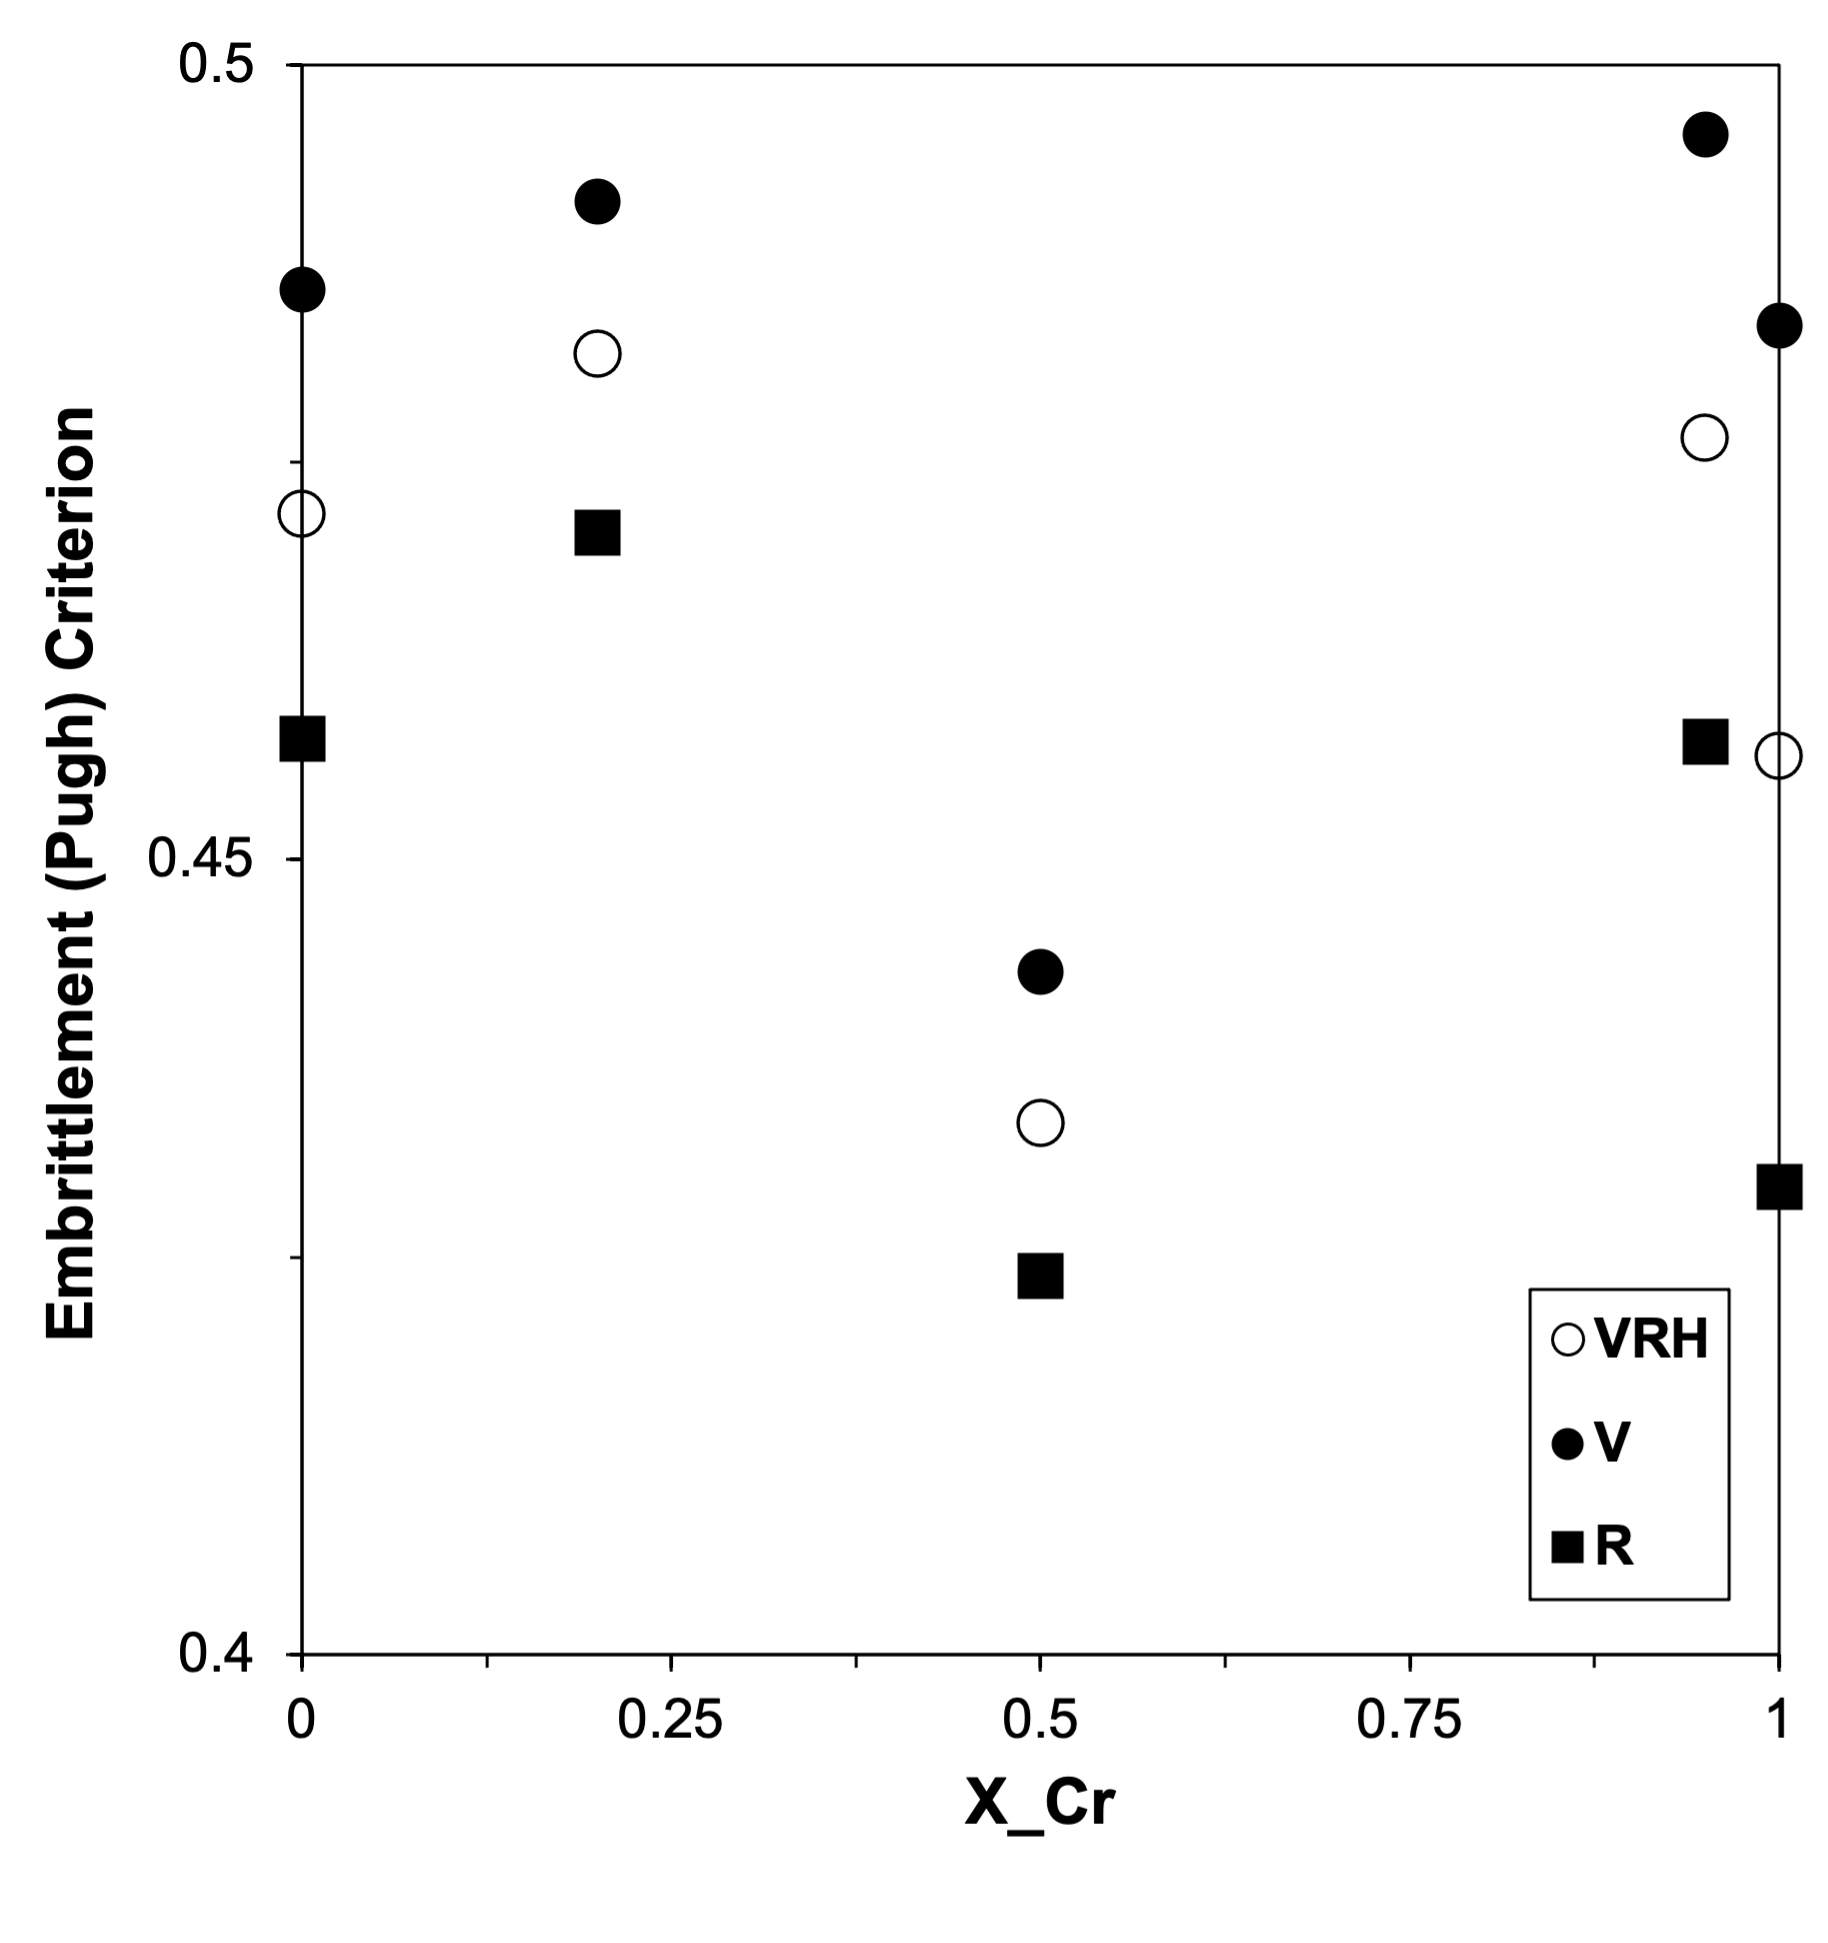
\includegraphics[width=\linewidth]{Parts/Figures/EvsX_vF.png}
         \caption{Embrittlement (Pugh) Criterion, calculated to evaluate the embrittlement risk associated with varying Cr compositions.}
         \label{fig3d}
     \end{subfigure}
	\caption{(a) The enthalpy of mixing demonstrates the thermodynamic drive towards phase separation indicative of spinodal decomposition, affecting the material's mechanical integrity. (b) Variations in the melting temperature as a function of Cr composition offer insights into the thermal stability and potential phase transformations within the alloy. (c) Changes in Rayleigh wave frequencies across compositions highlight alterations in surface acoustic properties, correlating with mechanical behavior. (d) The Embrittlement (Pugh) Criterion allows for assessing the risk of material embrittlement due to changes in composition, crucial for ensuring material reliability in critical applications.}
	\label{fig3}
\end{sidewaysfigure}


\begin{sidewaysfigure}[!ht]
    \centering
    \begin{subfigure}{0.9\textwidth}
        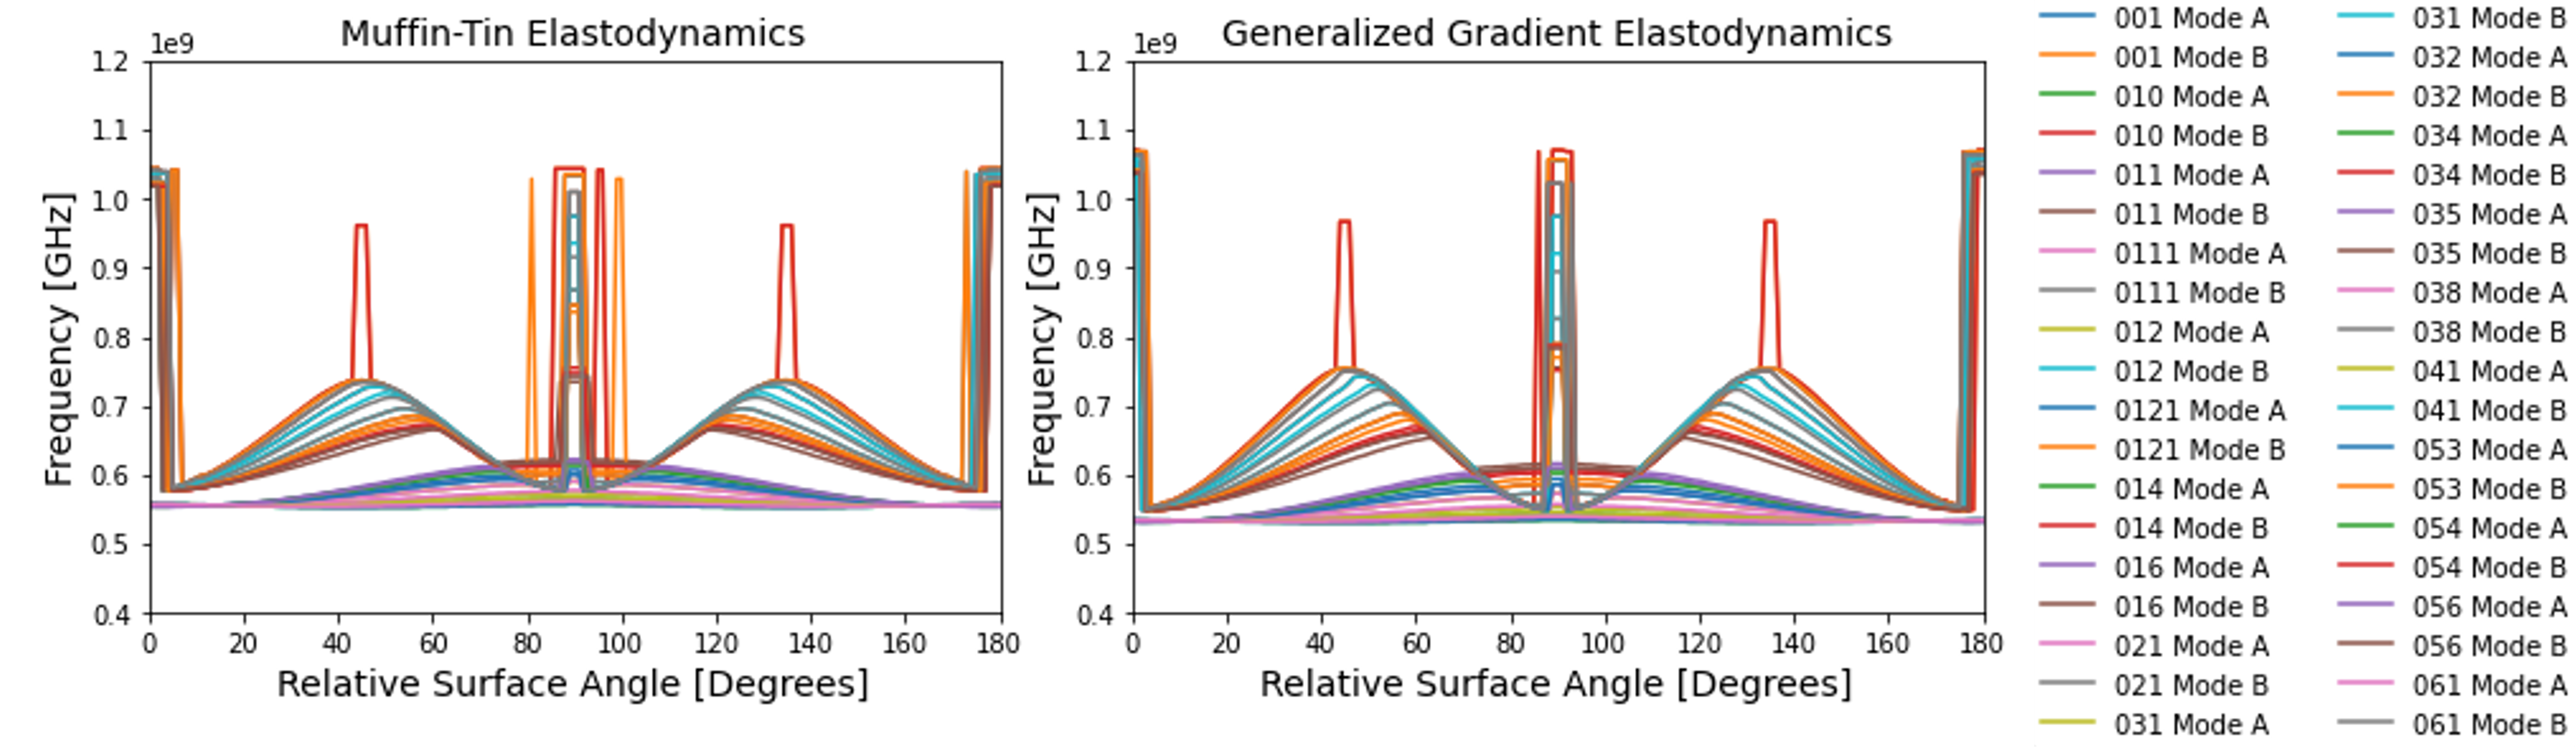
\includegraphics[width=\textwidth]{Parts/Figures/smoking-gun-v2.png}
        \caption{Predicted elastic frequencies showcasing the emergence of new modes within the elastodynamically-unallowed regions, signifying alterations in the material's mechanical properties due to spinodal decomposition. These frequencies match closely with experimentally observed values in aged stainless steel specimens, providing a quantum mechanical insight into the microstructural evolution impacting material performance.}
        \label{fig4a}
    \end{subfigure}
    \begin{subfigure}{0.35\textwidth}
        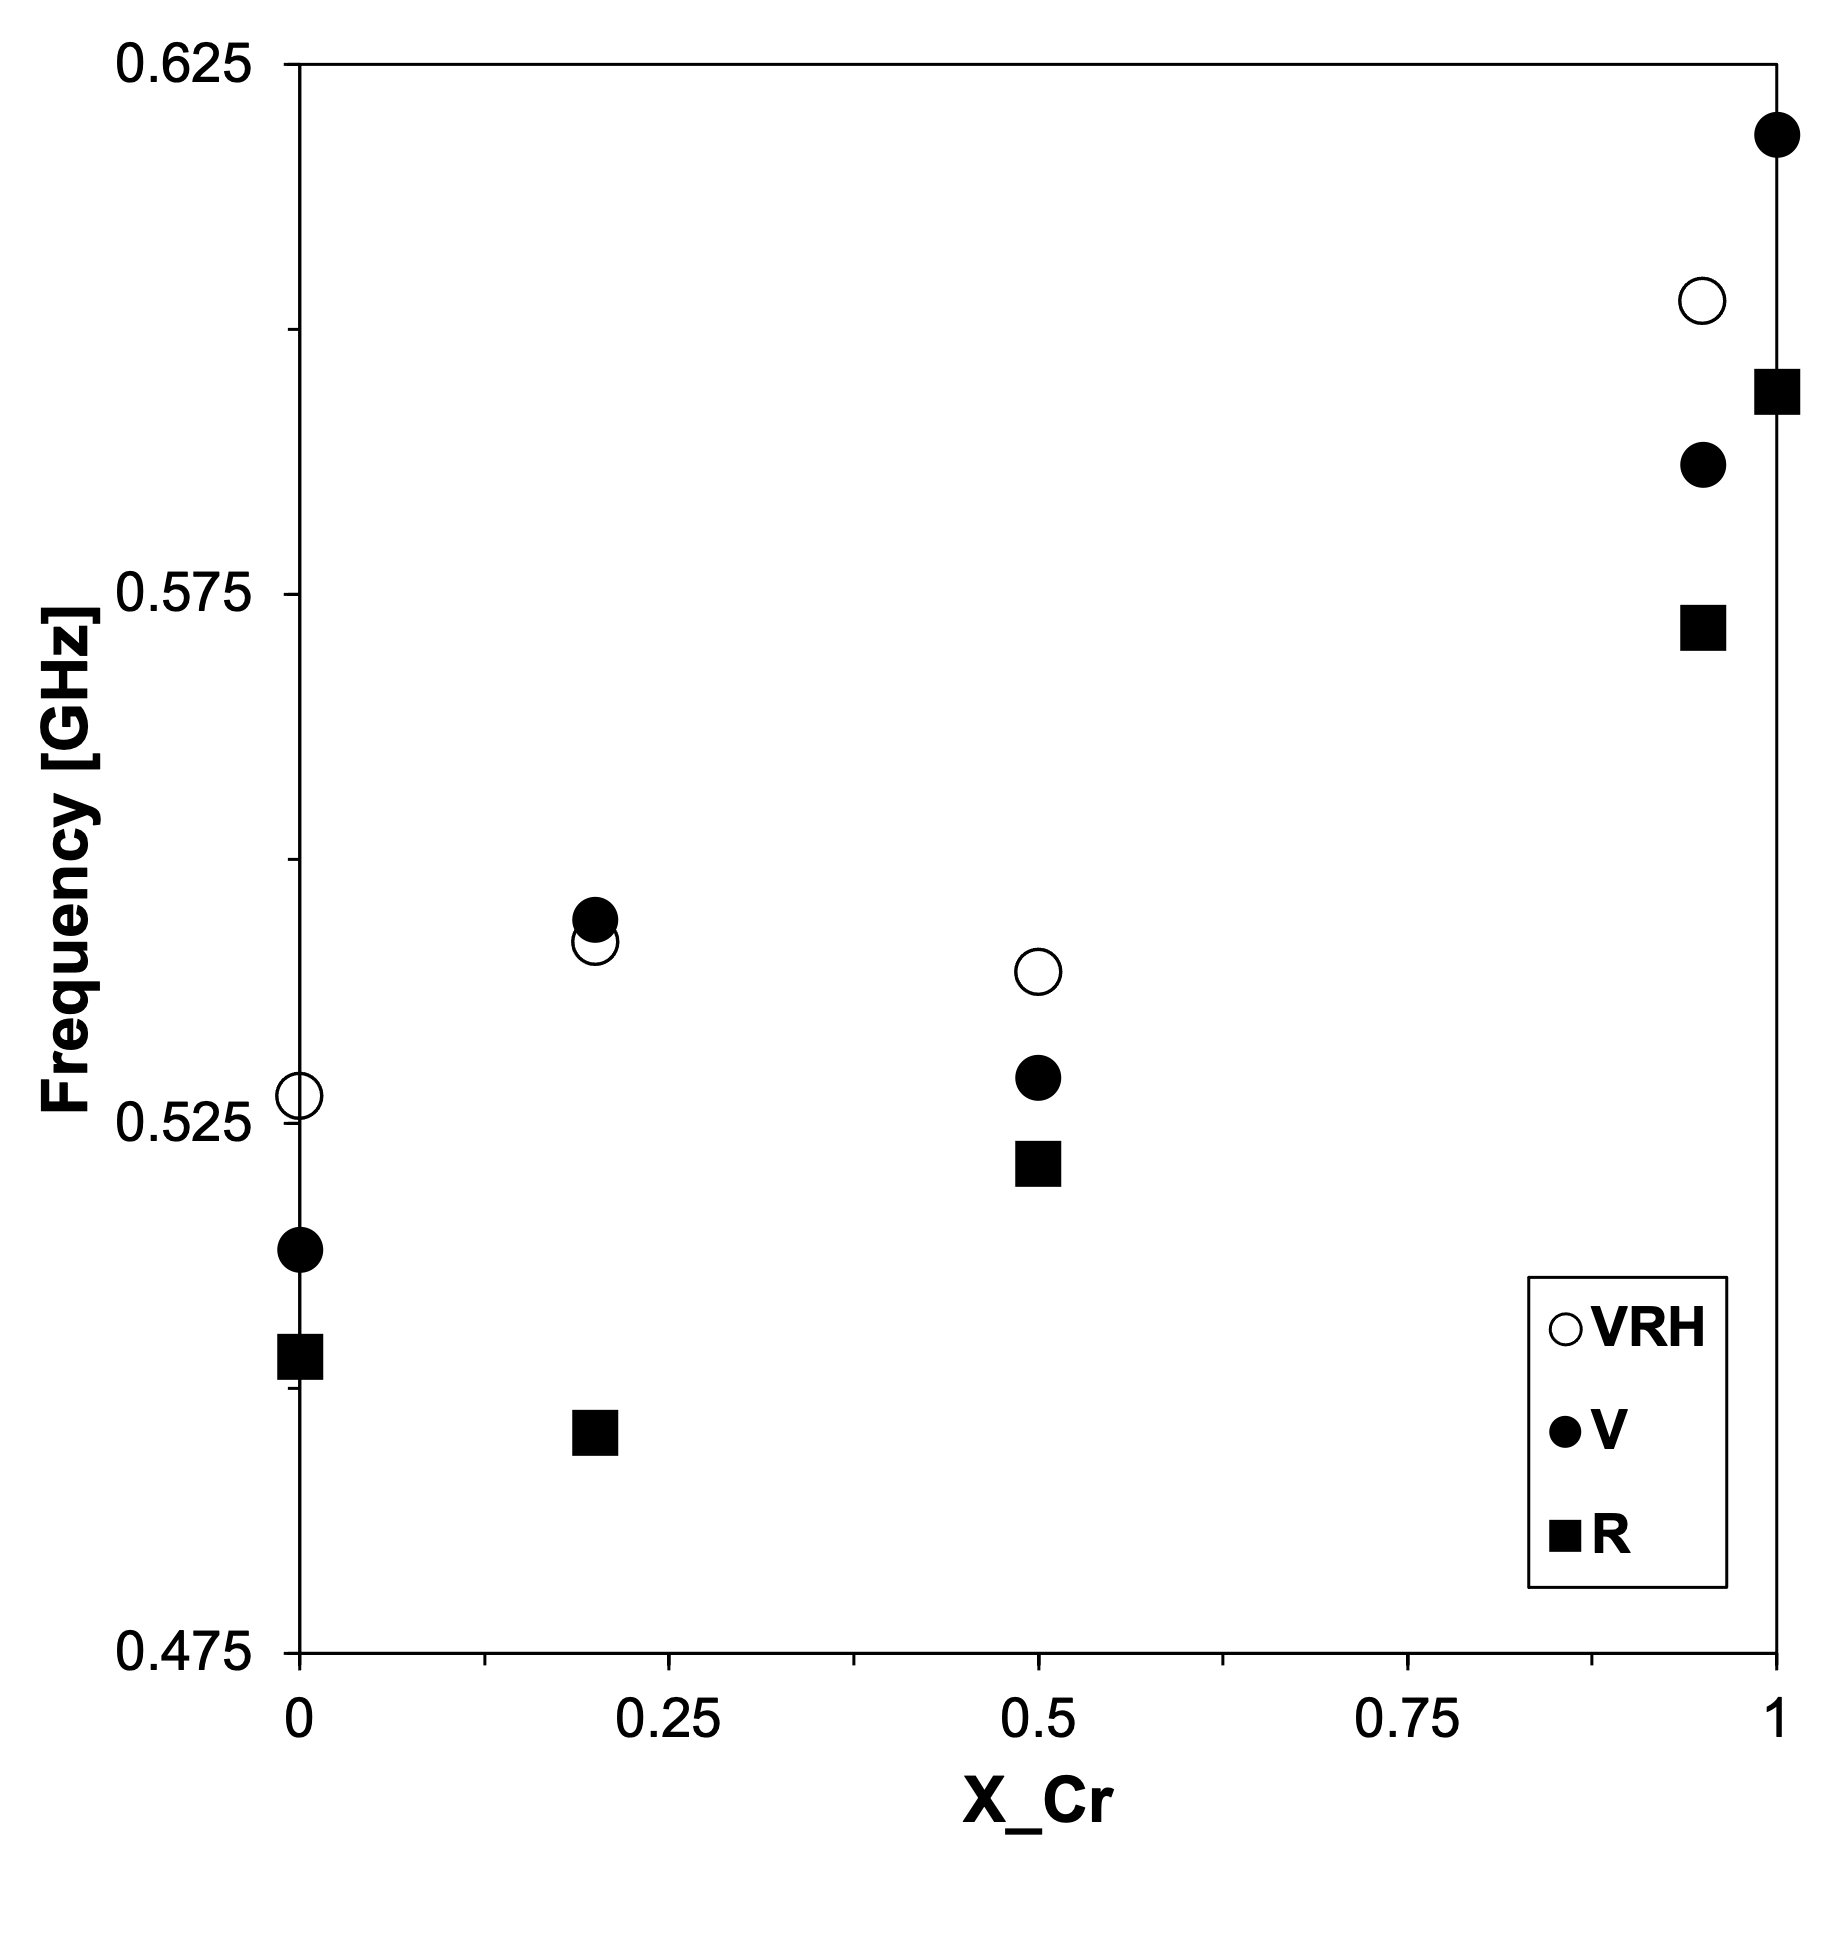
\includegraphics[width=\textwidth, left]{Parts/Figures/fvsX_v3.png}
        \caption{Calculated acoustic frequencies across different Cr compositions, illustrating the material's acoustic response variability with composition. This graph provides a quantitative measure of the material's mechanical behavior and its dependence on the microstructural characteristics induced by varying chromium content.}
        \label{fig4b}
    \end{subfigure}
    \begin{subfigure}{0.5\textwidth}
        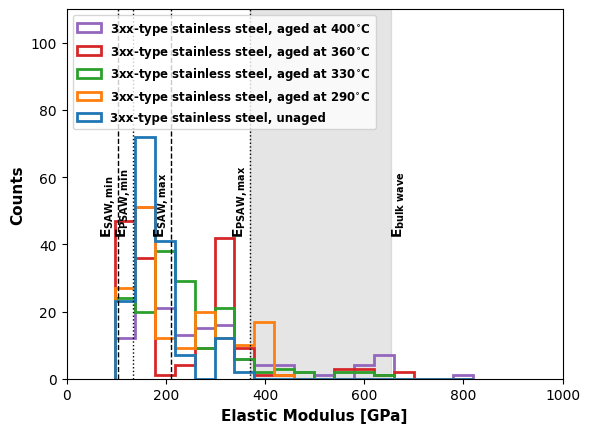
\includegraphics[width=\textwidth, right]{Parts/Figures/experimental-moduli-hist.png}
        \caption{Measured elastic moduli distribution from experimental data, highlighting the range and variability of material properties within stainless steel samples subjected to different thermal aging processes. The distribution underscores the significant impact of microstructural changes, such as spinodal decomposition, on the material's overall stiffness and mechanical integrity.}
        \label{fig4c}
    \end{subfigure}
    \caption{(a) Quantum elastodynamic frequencies obtained from density functional theory calculations reveal the complex interplay between microstructural evolution and mechanical properties in stainless steels undergoing spinodal decomposition. These findings are corroborated by (b) calculated acoustic frequencies that vary with Cr composition, providing a link between composition, microstructure, and acoustic properties. (c) The distribution of measured elastic moduli further validates the theoretical predictions, illustrating the broad impact of aging and compositional changes on the material's mechanical performance.}
    \label{fig4}
\end{sidewaysfigure}


\begin{sidewaysfigure}[!ht]
	\centering
	\begin{subfigure}{0.3\textwidth}
         \centering
         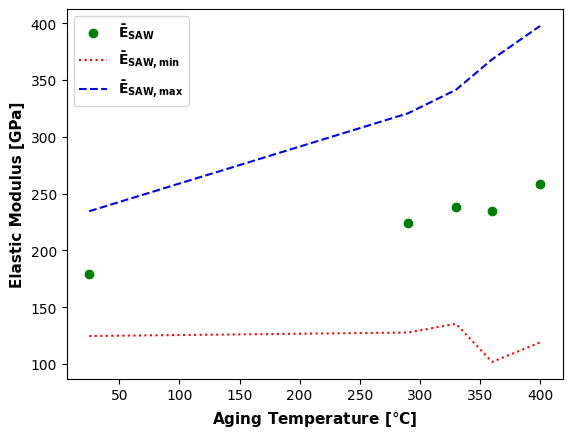
\includegraphics[width=\linewidth]{Parts/Figures/experimental-moduli-trend.png}
         \caption{Experimental elastic moduli of aged steels, displaying how aging temperature influences the material's stiffness. This graph illustrates the correlation between thermal treatment and the increase in elastic moduli, indicative of the material's response to microstructural changes over time.}
         \label{fig5a}
     \end{subfigure}
     \hfill
     \begin{subfigure}{0.3\textwidth}
         \centering
         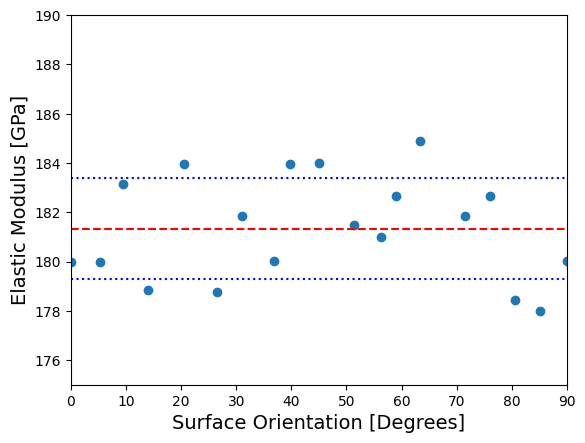
\includegraphics[width=\linewidth]{Parts/Figures/approximate-elastic-moduli-from-SAW-measurements-pristine.png}
         \caption{Theoretical elastic moduli of pristine steels, offering a baseline comparison for understanding how spinodal decomposition affects material properties before and after aging. This comparison elucidates the stiffening effect of microstructural evolution on the alloy's mechanical behavior.}
         \label{fig5b}
     \end{subfigure}
     \hfill
     \begin{subfigure}{0.3\textwidth}
         \centering
         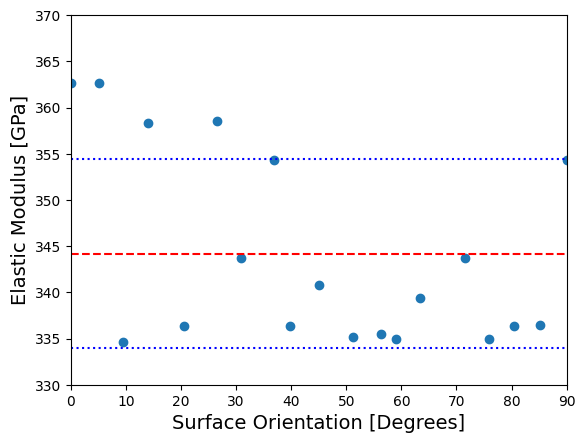
\includegraphics[width=\linewidth]{Parts/Figures/approximate-elastic-moduli-from-SAW-measurements-spindec.png}
         \caption{Theoretical elastic moduli of spinodally decomposed steels, demonstrating the pronounced impact of microstructural evolution on the alloy's stiffness. This direct comparison to pristine conditions highlights the significant role of chromium composition and thermal aging in material performance.}
         \label{fig5c}
     \end{subfigure}
     \hfill
     \begin{subfigure}{0.3\textwidth}
         \centering
         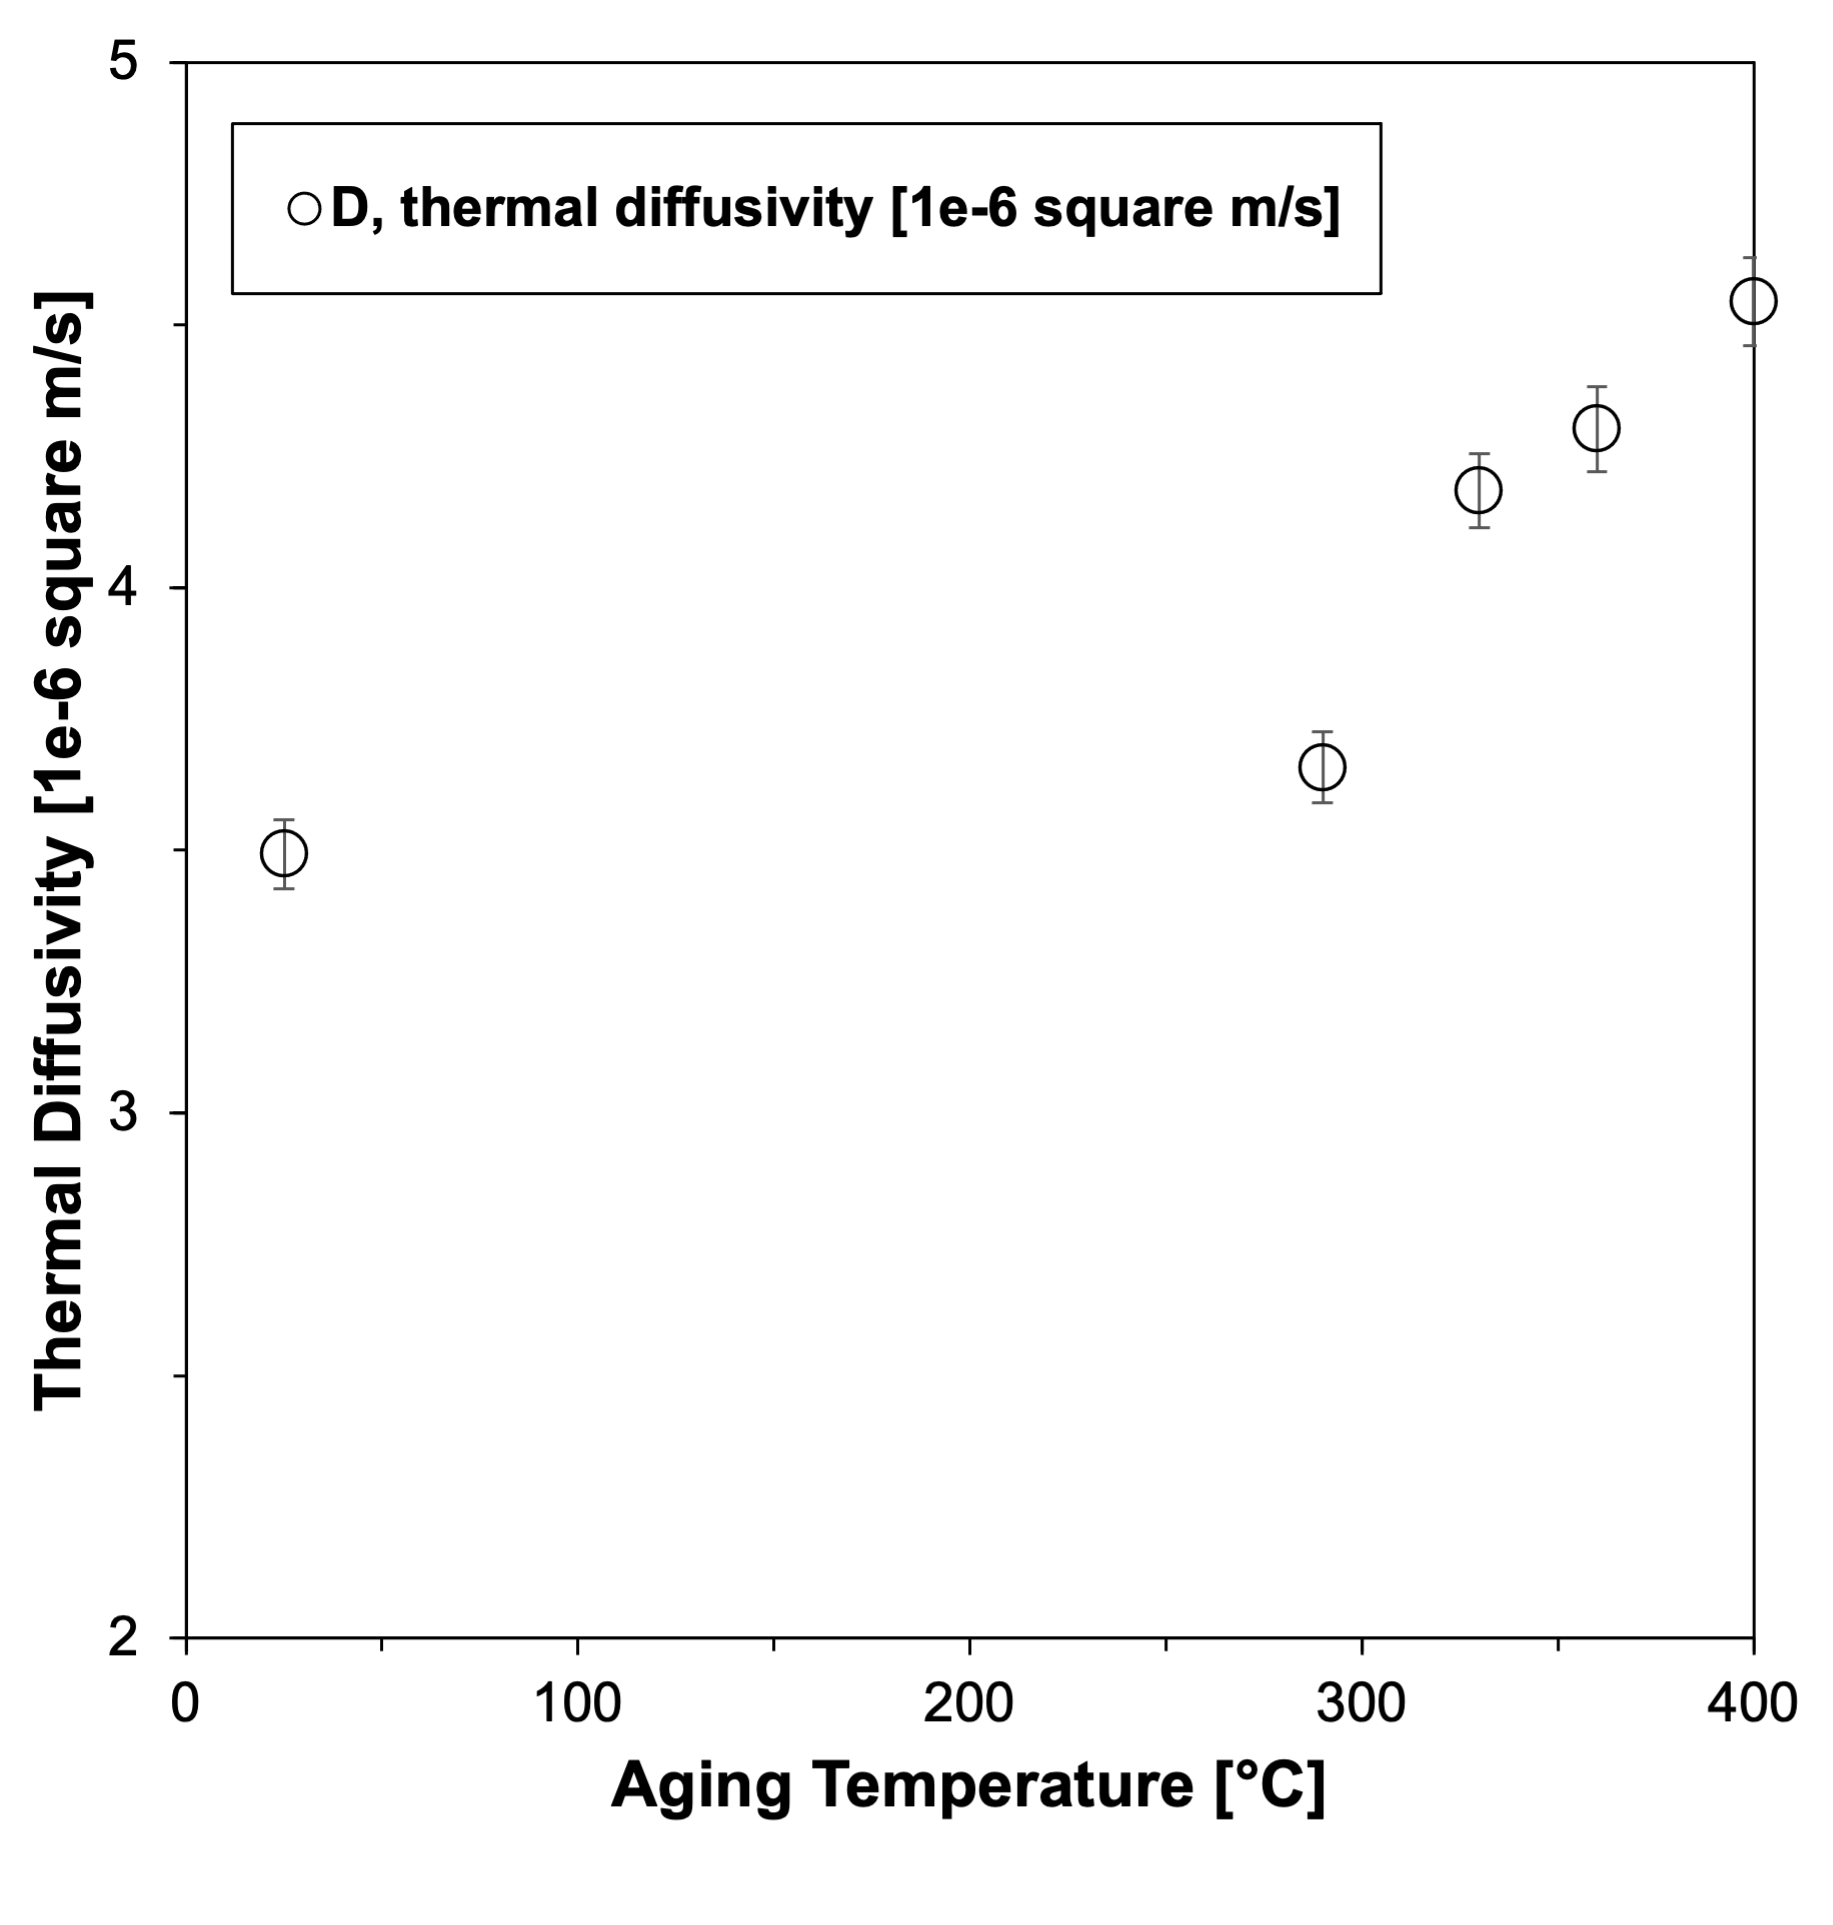
\includegraphics[width=\linewidth]{Parts/Figures/DvsT_CF8_30khrs_v2.png}
         \caption{\(D^{exp}_{thermal}\), experimental thermal diffusivity as measured in aged stainless steel, illustrating the thermal transport characteristics and their variation with temperature. This metric provides insights into the thermal stability and heat dissipation capabilities of the material post-aging.}
         \label{fig5d}
     \end{subfigure}
     \hfill
     \begin{subfigure}{0.3\textwidth}
         \centering
         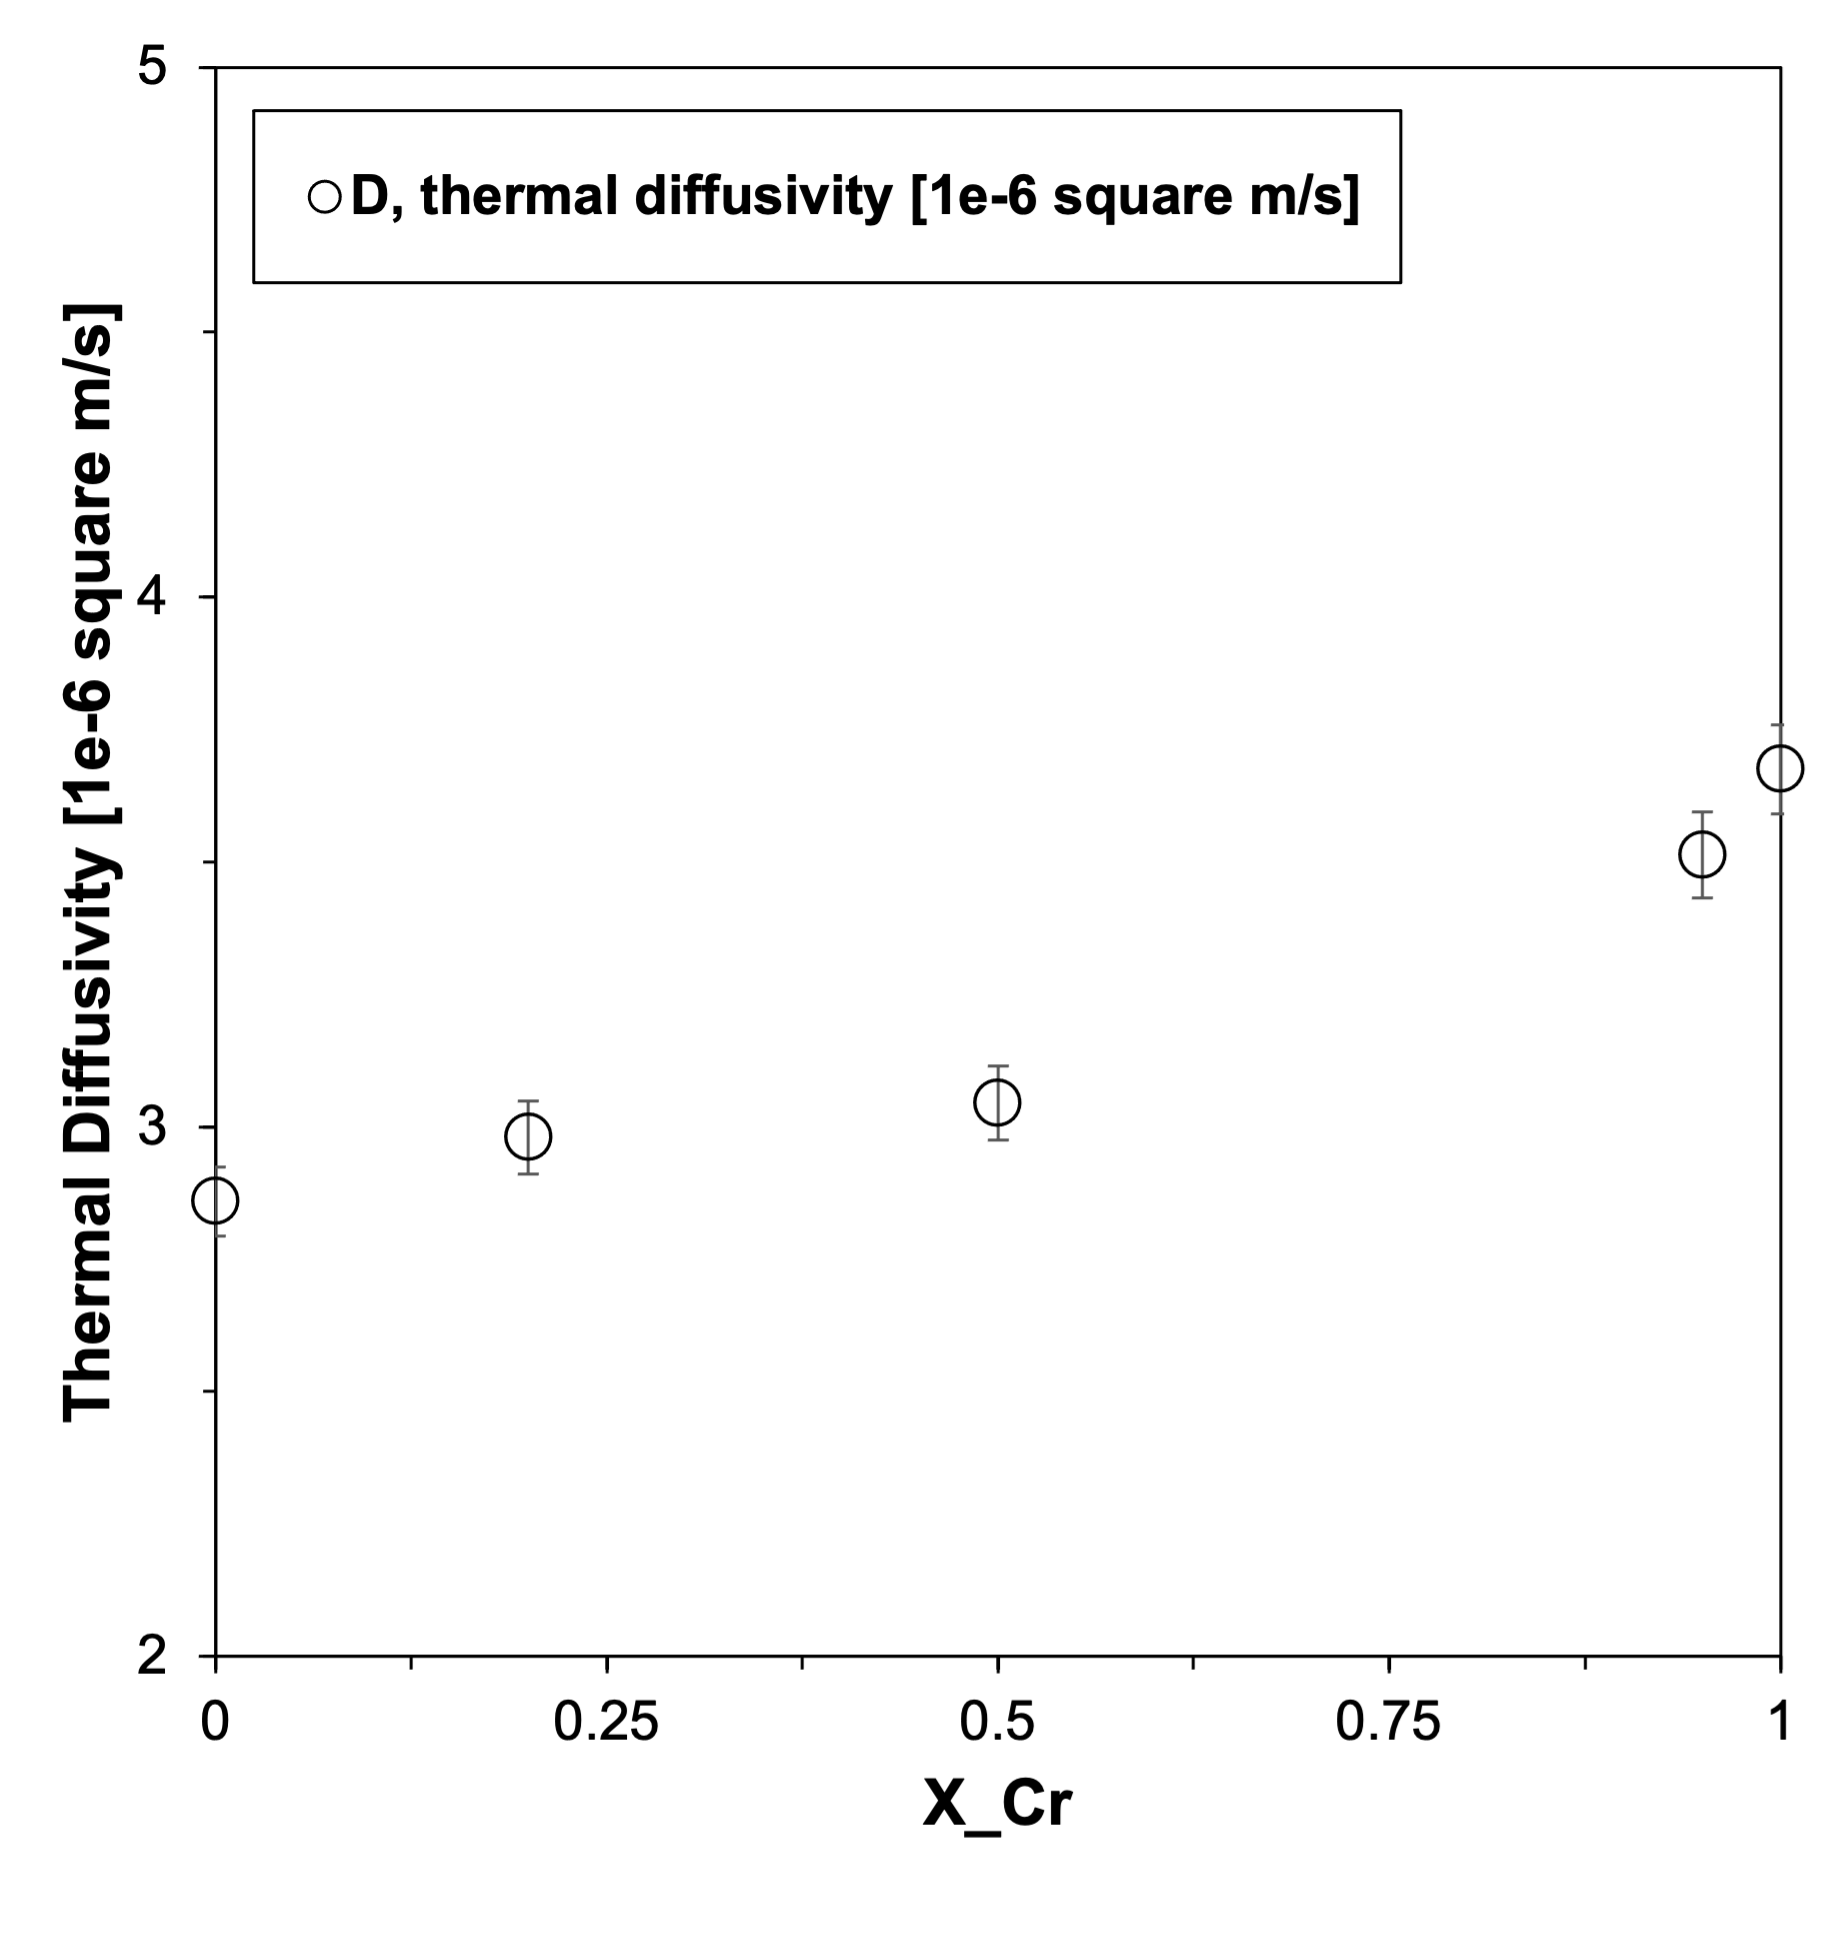
\includegraphics[width=\linewidth]{Parts/Figures/DvsX_v4.png}
         \caption{\(D^{theoretical}_{thermal}\), theoretical thermal diffusivity indicating the expected thermal behavior based on composition and microstructural considerations. This predictive analysis aids in understanding the thermal management potential of the alloy across a range of compositions.}
         \label{fig5e}
     \end{subfigure}
     \hfill
     \begin{subfigure}{0.3\textwidth}
         \centering
         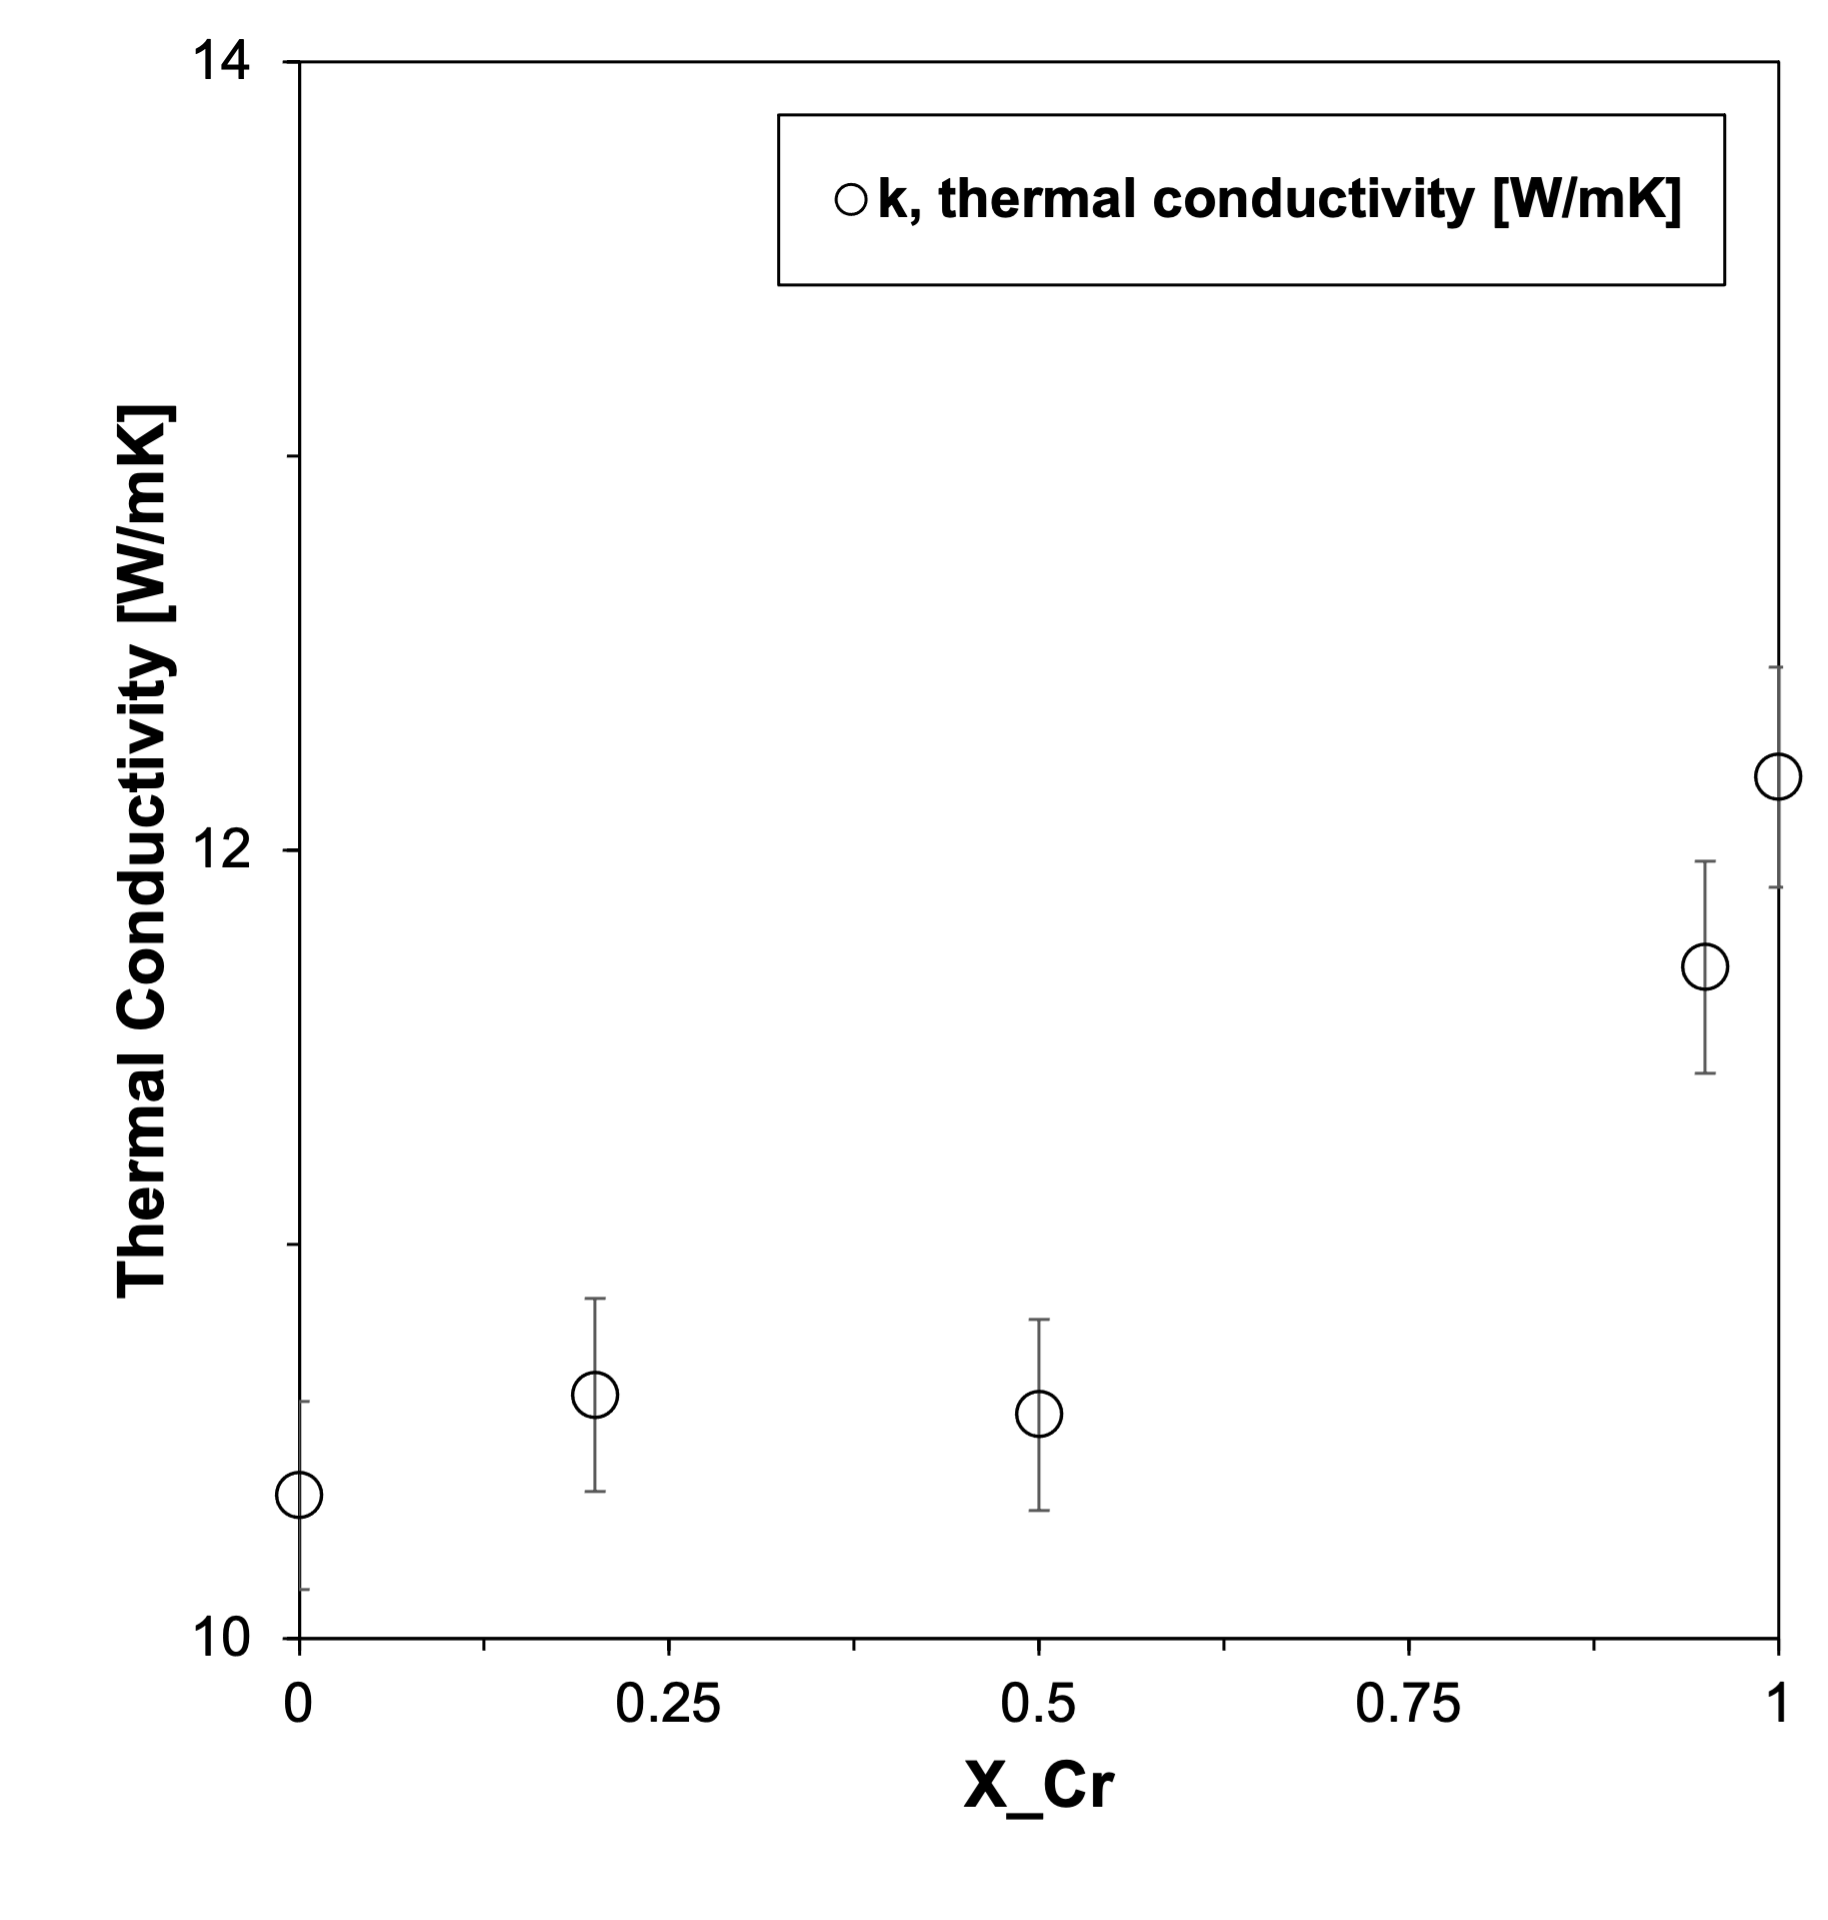
\includegraphics[width=\linewidth]{Parts/Figures/KvsX_v2.png}
         \caption{\(\kappa^{theoretical}_{thermal}\), thermal conductivity, showcasing the theoretical prediction of how efficiently the material conducts heat. This property is crucial for applications where thermal management is key, and it is influenced by the alloy's microstructure and composition.}
         \label{fig5f}
     \end{subfigure}
	\caption{Comprehensive analysis combining experimental and theoretical insights into the thermal and mechanical properties of stainless steels subjected to thermal aging. (a) Experimental elastic moduli trends with aging temperature highlight the stiffening effect of microstructural evolution. (b) and (c) Theoretical predictions for pristine and spinodally decomposed steels provide a comparative framework for assessing the impact of spinodal decomposition on material properties. (d) Experimental thermal diffusivity measurements, alongside (e) theoretical predictions for thermal diffusivity and (f) thermal conductivity, offer a holistic view of the material's thermal and mechanical behavior post-aging, emphasizing the interconnectedness of thermal properties, mechanical performance, and microstructural characteristics.}
	\label{fig5}
\end{sidewaysfigure}


\end{document}
